\documentclass[aps,prd,reprint,preprintnumbers,showpacs,floatfix,nofootinbib,superscript address]{revtex4-2}
\usepackage[utf8]{inputenc}
\usepackage{amssymb}
\usepackage{stix}
\usepackage{amsmath}
\usepackage{mathtools}
\usepackage[dvipsnames]{xcolor}
\usepackage{xspace}
\usepackage{siunitx}
\usepackage{multirow}
\usepackage{graphicx}
\usepackage{xstring}
\usepackage{etoolbox}
\usepackage{notoccite}
\usepackage{natbib}
\usepackage{mathrsfs}
\usepackage{lineno}
\usepackage{tensor}
\usepackage{accents}
\allowdisplaybreaks
\DeclareSIUnit\parsec{pc}

%MacrosTextual

\usepackage{xspace}
\usepackage{xstring}
\usepackage{titlesec}
%\usepackage{parskip}
\usepackage{stix}
\usepackage{soul}
\allowdisplaybreaks
%\parskip 1mm
%\parindent 2mm

%	Basic abbreviations
\newcommand*{\ie}{i.e., }
\newcommand*{\eg}{e.g., }
\newcommand*{\fig}{fig.\@\xspace}
\newcommand*{\eq}{eq.\@\xspace}
\newcommand*{\eqs}{eqs.\@\xspace}
\newcommand*{\wrt}{w.r.t.\@\xspace}

%	Comments
\newcommand{\sz}[1]{{\color[RGB]{0,34,170}{#1}}}
\newcommand{\wb}[1]{{\color[RGB]{0,100,154}{#1}}}
\newcommand{\wbn}[1]{{\color[RGB]{0,100,154}{[WB narrative: ``\textit{#1}'']}}}
\newcommand{\szC}[1]{{\color[RGB]{0,34,170}{[\textbf{SZ: #1]}}}}

%	PRL paragraph
\newrobustcmd{\pea}[1]{%
	\emph{#1}\textbf{\ \ \ ---}
}
\titleformat{\paragraph}[runin]{\normalfont\normalsize\bfseries}{\emph\theparagraph}{1em}{\pea}

% Highlight edits
\newcommand{\myDel}[1]{{\color{red}\ifmmode\cancel{#1}\else\st{#1}\fi}}
\newcommand{\myNew}[1]{{\color{red}#1}}
\newcommand{\myRe}[2]{\myDel{#1} \myNew{#2}}
\newcommand{\myTODO}[1]{{\color{brown}#1}}

% Numerical fractions
\def\tfrac#1#2{{\textstyle\frac{#1}{#2}}}



%MacrosMAG

\usepackage{etoolbox}
\usepackage{tensor}

\newrobustcmd{\PSALTer}{\textit{PSALTer}\xspace}
\newrobustcmd{\MPl}{%
	{m_{\mathrm{P}}} 
}
\newrobustcmd{\LPl}{%
	{\ell_{\mathrm{P}}} 
}
\newrobustcmd{\LPhy}{%
{\ell_{\mathrm{Phy}}} 
}
\newrobustcmd{\LPhyprime}{%
{\ell^\prime_{\mathrm{Phy}}} 
}
\newrobustcmd{\FieldOmega}[1]{%
  \tensor{\omega}{#1}
}
\newrobustcmd{\FieldTau}[1]{%
  \tensor{\tau}{#1}
}
\newrobustcmd{\FieldSpin}[1]{%
  \tensor{\sigma}{#1}
}
\newrobustcmd{\FieldPert}[1]{%
  \tensor{f}{#1}
}
\newrobustcmd{\FieldMomentum}[1]{%
  \tensor{k}{#1}
}
\newrobustcmd{\FieldVScalar}[1]{%
  \tensor{\delta B_\perp}{#1}
}
\newrobustcmd{\FieldVScalarDagger}[1]{%
  \tensor{\delta B_\perp^*}{#1}
}
\newrobustcmd{\FieldVVector}[1]{%
  \tensor{\delta B_\parallel}{#1}
}
\newrobustcmd{\FieldVVectorDagger}[1]{%
  \tensor{\delta B_\parallel^*}{#1}
}
\newrobustcmd{\FieldF}[1]{%
  \tensor{F}{#1}
}
\newrobustcmd{\SCovD}[1]{%
	\tensor{\mathscr{D}}{#1}
}
\newrobustcmd{\FieldH}[1]{%
  \tensor{h}{#1}
}
\newrobustcmd{\FieldHHat}[1]{%
  \tensor{\hat h}{#1}
}
\newrobustcmd{\FieldB}[1]{%
  \tensor{b}{#1}
}
\newrobustcmd{\FieldBHat}[1]{%
  \tensor{\hat b}{#1}
}
\newrobustcmd{\FieldV}[1]{%
  \tensor{B}{#1}
}
\newrobustcmd{\FieldVHat}[1]{%
  \tensor{\hat B}{#1}
}
\newrobustcmd{\FieldVV}[1]{%
  \tensor{V}{#1}
}
\newrobustcmd{\FieldSigma}[1]{%
  \tensor{\Sigma}{#1}
}
\newrobustcmd{\FieldATilde}[1]{%
  \tensor{\tilde A}{#1}
}
\newrobustcmd{\Curtright}[1]{%
  \tensor{C}{#1}
}
\newrobustcmd{\FieldAHat}[1]{%
  \tensor{\hat A}{#1}
}
\newrobustcmd{\Alp}[1]{%
  \tensor{\alpha}{_#1}
}
\newrobustcmd{\Bet}[1]{%
  \tensor{\beta}{_#1}
}
\newrobustcmd{\Gam}[1]{%
  \tensor{\gamma}{_#1}
}
\newrobustcmd{\MassSquared}[1]{%
	\left(\tensor{m}{_{#1}}\right)^2
}
\newrobustcmd{\FieldA}[1]{%
  \tensor{A}{#1}
}
\newrobustcmd{\FieldDelta}[1]{%
	\tensor*{\delta}{#1}
}
\newrobustcmd{\FieldEta}[1]{%
	\tensor{\eta}{#1}
}
\newrobustcmd{\FieldX}[1]{%
	\tensor{x}{#1}
}
\newrobustcmd{\FieldY}[1]{%
	\tensor{y}{#1}
}
\newrobustcmd{\FieldG}[1]{%
	\tensor{g}{#1}
}
\newrobustcmd{\FieldGHat}[1]{%
	\tensor{\hat g}{#1}
}
\newrobustcmd{\FieldLambda}[1]{%
	\tensor{\Lambda}{#1}
}
\newrobustcmd{\PD}[1]{%
	\tensor{\partial}{#1}%
}
\newrobustcmd{\Danger}[1]{%
	{\color{red}{#1}}	
}
\newrobustcmd{\Coupling}[1]{%
	{a_{#1}}	
}
\newrobustcmd{\CouplingB}[1]{%
	{b_{#1}}	
}
\newrobustcmd{\MAGg}[1]{%
	\tensor{g}{#1}
}
\newrobustcmd{\MAGl}[1]{%
	\tensor{\xi}{#1}
}
\newrobustcmd{\MAGP}[1]{%
  \tensor{P}{#1}
}
\newrobustcmd{\MAGC}[1]{%
  \tensor{C}{#1}
}
\newrobustcmd{\ShiftA}[1]{%
  \tensor{A}{#1}
}
\newrobustcmd{\ShiftB}[1]{%
  \tensor{B}{#1}
}
\newrobustcmd{\ShiftC}[1]{%
  \tensor{C}{#1}
}
\newrobustcmd{\MAGA}[1]{%
  \tensor{\Gamma}{#1}
}
\newrobustcmd{\Ja}[1]{%
	\tensor{\smash{\overset{\scalebox{0.6}{$\mathrm{(M)}$}}{\mathcal{J}}}}{#1}
}
\newrobustcmd{\Jv}[1]{%
	\tensor{\smash{\overset{\scalebox{0.6}{$\mathrm{(N)}$}}{\mathcal{J}}}}{#1}
}
\newrobustcmd{\MAGH}[1]{%
	\tensor{H}{#1}
}
\newrobustcmd{\MAGHHat}[1]{%
	\tensor{\hat H}{#1}
}
\newrobustcmd{\MAGF}[1]{%
	\tensor{R}{#1}
}
\newrobustcmd{\MAGFt}[1]{%
	\tensor{\tilde{R}}{#1}
}
\newrobustcmd{\MAGFh}[1]{%
	\tensor{\hat{R}}{#1}
}
\newrobustcmd{\MAGFa}[1]{%
	\tensor{\check{R}}{#1}
}
\newrobustcmd{\MAGFb}[1]{%
	\tensor{R}{#1}
}
\newrobustcmd{\MAGT}[1]{%
	\tensor{T}{#1}
}
\newrobustcmd{\MAGTTilde}[1]{%
	\tensor{\tilde T}{#1}
}
\newrobustcmd{\MAGTt}[1]{%
	\tensor{\hat{T}}{#1}
}
\newrobustcmd{\MAGt}[1]{%
	\tensor{t}{#1}
}
\newrobustcmd{\MAGQ}[1]{%
	\tensor{Q}{#1}
}
\newrobustcmd{\MAGQt}[1]{%
	\tensor{\hat{Q}}{#1}
}
\newrobustcmd{\MAGq}[1]{%
	\tensor{q}{#1}
}
\newrobustcmd{\MAGV}[1]{%
	\tensor{Z}{#1}
}
\newrobustcmd{\MAGVt}[1]{%
	\tensor{\tilde{Z}}{#1}
}


\newrobustcmd{\xMAGA}[1]{%
  \tensor{A}{#1}
}
\newrobustcmd{\xMAGF}[1]{%
	\tensor{\mathcal{F}}{#1}
}
\newrobustcmd{\xMAGFt}[1]{%
	\tensor{\tilde{\mathcal{F}}}{#1}
}
\newrobustcmd{\xMAGFa}[1]{%
	\tensor{\mathcal{F}}{^{(14)}#1}
}
\newrobustcmd{\xMAGFb}[1]{%
	\tensor{\mathcal{F}}{^{(13)}#1}
}
\newrobustcmd{\xMAGT}[1]{%
	\tensor{\mathcal{T}}{#1}
}
\newrobustcmd{\xMAGTt}[1]{%
	\tensor{\tilde{\mathcal{T}}}{#1}
}
\newrobustcmd{\xMAGQ}[1]{%
	\tensor{\mathcal{Q}}{#1}
}
\newrobustcmd{\xMAGQt}[1]{%
	\tensor{\tilde{\mathcal{Q}}}{#1}
}
\newrobustcmd{\xMAGTh}[1]{%
	\tensor{\hat{\mathcal{T}}}{#1}
}
\newrobustcmd{\xMAGV}[1]{%
	\tensor{\mathcal{V}}{#1}
}
\newrobustcmd{\g}[1]{%
	\tensor{g}{#1}%
}
\newrobustcmd{\rcCon}[1]{%
	\tensor*{\Gamma}{#1}%
}
\newrobustcmd{\rCon}[1]{%
	\tensor{\mathring{\Gamma}}{#1}%
}
\newrobustcmd{\Con}[1]{%
	\tensor{\mathring{\Gamma}}{#1}%
}
\newrobustcmd{\B}[1]{%
	\tensor{B}{#1}%
}
\newrobustcmd{\rD}[1]{%
	\tensor{\mathring{\nabla}}{#1}%
}
\newrobustcmd{\rcD}[1]{%
	\tensor{\nabla}{#1}%
}
\newrobustcmd{\rR}[1]{%
	\tensor{\mathring{R}}{#1}%
}
\newrobustcmd{\rcR}[1]{%
	\tensor{R}{#1}%
}

\input{MacrosJournalNames.tex}

\usepackage{hyperref}
\hypersetup{%
     colorlinks = true,%
     linkcolor = Blue,%
     citecolor = Blue,%
     filecolor = Blue,%
     urlcolor = Blue% 
     }%

\usepackage[capitalize]{cleveref}

\usepackage{layouts}

\begin{document}

\title{Every Poincar\'e gauge theory is conformal: a compelling case for dynamical vector torsion}

\author{Will Barker}
\email{wb263@cam.ac.uk}
\affiliation{Astrophysics Group, Cavendish Laboratory, JJ Thomson Avenue, Cambridge CB3 0HE, UK}
\affiliation{Kavli Institute for Cosmology, Madingley Road, Cambridge CB3 0HA, UK}

\author{Michael Hobson}
\email{mph13@cam.ac.uk}
\affiliation{Astrophysics Group, Cavendish Laboratory, JJ Thomson Avenue, Cambridge CB3 0HE, UK}

\author{Anthony Lasenby}
\email{a.n.lasenby@mrao.cam.ac.uk}
\affiliation{Astrophysics Group, Cavendish Laboratory, JJ Thomson Avenue, Cambridge CB3 0HE, UK}
\affiliation{Kavli Institute for Cosmology, Madingley Road, Cambridge CB3 0HA, UK}

\author{Yun-Cherng Lin}
\email{yunclin54@gmail.com}
\affiliation{Astrophysics Group, Cavendish Laboratory, JJ Thomson Avenue, Cambridge CB3 0HE, UK}
\affiliation{Kavli Institute for Cosmology, Madingley Road, Cambridge CB3 0HA, UK}

\author{Zhiyuan Wei}
\email{zhiyuan.wei@uni-ulm.de}
\affiliation{Astrophysics Group, Cavendish Laboratory, JJ Thomson Avenue, Cambridge CB3 0HE, UK}
\affiliation{Institute for Complex Quantum Systems, Ulm University, Albert-Einstein-Allee, 89069 Ulm, DE}

\begin{abstract}
	The Poincar\'e gauge theory (PGT) of gravity provides a viable formulation of general relativity (Einstein--Cartan theory), and a popular model-building framework for modified gravity with torsion. Notoriously, however, the PGT terms which propagate vector torsion lead to strongly-coupled ghosts: the modern view is that only scalar torsion can propagate. To fix this, we revisit the concept of embedding explicit mass scales in scale-invariant theories, showing how the Klein--Gordon theory naturally leads to a slowly-rolling inflaton. We then show that the unique scale-invariant embedding of PGT leads to two new terms, one of which is the Maxwell term for vector torsion. We provide the full spectrum of quantum particles in the resulting theory. Our result means that every PGT is conformal and -- after a two-decade hiatus -- vector torsion is back on the menu.
\end{abstract}

\maketitle

\paragraph*{Introduction to torsion} General relativity (GR) offers a remarkably successful description of gravity as spacetime curvature~\cite{Einstein:1915}.\footnote{The term `GR' refers strictly to the textbook, metric-based theory with an Einstein--Hilbert action in Riemann spacetime.} An open problem is the degree -- if any -- to which spacetime \emph{torsion} also participates in the gravitational interaction. There are excellent theoretical reasons to consider torsion: it was shown by Utiyama~\cite{Utiyama:1956sy}, Kibble~\cite{Kibble:1961ba} and Sciama~\cite{Sciama:1962} that when fermions are coupled to gravity, the natural result is a local gauge theory not only of spacetime translations (i.e. the diffeomorphisms of GR), but also of spatial rotations and Lorentz boosts. In this \emph{Poincar\'e gauge theory} (PGT) of gravity~\cite{Blagojevic:2002}, the fundamental fields can be\footnote{By contrast with GR, the term `PGT' encompasses \emph{any} action formulated with the 40 d.o.f of the tetrad and spin connection in Riemann--Cartan spacetime. In the absence of fermionic matter, the dynamics of PGT are also fully captured by the alternative \emph{post-Riemannian} field parameterisation of 34 d.o.f in~$\big\{\FieldG{_{\mu\nu}},\MAGT{^\lambda_{\mu\nu}}\big\}$, though the Poincar\'e symmetry is hidden.} the metric tensor~$\FieldG{_{\mu\nu}}$ and an a priori independent affine connection~$\MAGA{^\alpha_{\mu}_{\nu}}$ which gives rise (as we will show later) to torsion and curvature as the field strength tensors of spacetime translations and rotations, respectively:
\begin{subequations}
\begin{align}
	\MAGT{^\alpha_\mu_\nu}&\equiv 2\MAGA{^\alpha_{[\mu}_{\nu]}},\label{ECTorsion}\\
	\MAGF{^\rho_\sigma_{\mu\nu}}&\equiv 2\left(\PD{_{[\mu|}}\MAGA{^\rho_{|\nu]}_\sigma}+\MAGA{^\rho_{[\mu|}_\alpha}\MAGA{^\alpha_{|\nu]}_\sigma}\right).\label{ECCurvature}
\end{align}
\end{subequations}
To connect this to textbook GR, if~$\MAGT{^\alpha_\mu_\nu}\to 0$ in~\cref{ECTorsion} then~$\MAGA{^\mu_\nu_\rho}$ loses its independence from the metric\footnote{We assume the metricity condition.} and is fixed by the Christoffel formula~$\MAGA{^\mu_\nu_\rho}\to\rCon{^\mu_{\nu\rho}}\equiv\FieldG{^{\mu\lambda}}\big(\PD{_{(\nu}}\g{_{\rho)\lambda}}-\frac{1}{2}\PD{_{\lambda}}\g{_{\nu\rho}}\big)$. In this torsion-free limit,~\cref{ECCurvature} defines the \emph{Riemannian} curvature~$\MAGF{^\rho_\sigma_{\mu\nu}}\to\rR{^\rho_\sigma_{\mu\nu}}$. Despite concrete theoretical provenance from PGT, there is uncertainty over what a signal for torsion might look like in the phenomena. This is in contrast to curvature, whose presence can be inferred e.g. through the geodesic motion of test particles. To understand this uncertainty, notice that we can always perform the field reparameterisation\footnote{Note~$\MAGA{^\mu_\nu_\rho}-\rCon{^\mu_\nu_\rho}$ is sometimes called \emph{contortion}, and is linear in torsion.}~$\MAGA{}\mapsto\rCon{}+\MAGT{}$ (leading to~$\MAGF{}\mapsto\rR{}+\PD{}\MAGT{}+\MAGT{}^2$ with indices suppressed). This \emph{post-Riemannian expansion} from variables~$\big\{\FieldG{_{\mu\nu}},\MAGA{^\alpha_{\mu}_{\nu}}\big\}$ to~$\big\{\FieldG{_{\mu\nu}},\MAGT{^\lambda_{\mu\nu}}\big\}$ reveals all PGT models to be nothing more than metric-based gravity coupled -- minimally or otherwise -- to the field~$\MAGT{^\lambda_{\mu\nu}}\equiv\MAGT{^\lambda_{[\mu\nu]}}$ as if it were an exotic kind of matter. Notice how there are infinitely many such models: if there are models for all experimental outcomes, then the theoretical framework ceases to be useful. The classic example of a useful PGT which establishes a predictive baseline is the minimal Einstein--Cartan theory (ECT)~\cite{Cartan:1922,Cartan:1923,Cartan:1924,Cartan:1925,Einstein:1925, Einstein:1928,Einstein:19282}. ECT is defined as the specific case of PGT which shares the Einstein--Hilbert action of GR
\begin{equation}\label{ECT}
	S_{\text{ECT}}\equiv\int\mathrm{d}^4x\sqrt{-g}\Big[-\frac{\MPl{}^2}{2}\MAGF{}
	-\MPl{}^2\Lambda+\text{matter}\Big],
\end{equation}
where~$\MAGF{}\equiv\MAGF{^\mu_\mu}\equiv\MAGF{^{\mu\nu}_{\mu\nu}}$ and~$\MPl{}\equiv 1/\sqrt{\kappa}$ is the Planck mass, for~$\kappa$ the Einstein constant. With~$\Lambda\equiv 0$ and in the absence of matter,~\cref{ECT} implies the vacuum Einstein equations~$\MAGF{_{\mu\nu}}= 0$ and the auxiliary equation~$\MAGT{^\lambda_{\mu\nu}}= 0$. Inclusion of matter leads to a contact spin-torsion coupling; the torsion integrates out to leave effective four-Fermi interactions~\cite{Kibble:1961ba, Rodichev:1961,Freidel:2005sn,Alexandrov:2008iy,Shaposhnikov:2020frq,Karananas:2021zkl,Rigouzzo:2023sbb}. Such interactions have many pheonomenological applications~\cite{Freidel:2005sn,Bauer:2008zj,Poplawski:2011xf,Diakonov:2011fs,Khriplovich:2012xg,Magueijo:2012ug,Khriplovich:2013tqa,Markkanen:2017tun,Carrilho:2018ffi,Enckell:2018hmo,Rasanen:2018fom,BeltranJimenez:2019hrm,Rubio:2019ypq,Shaposhnikov:2020geh,Karananas:2020qkp,Langvik:2020nrs,Shaposhnikov:2020gts,Mikura:2020qhc,Shaposhnikov:2020aen,Kubota:2020ehu,Enckell:2020lvn,Iosifidis:2021iuw,Bombacigno:2021bpk,Racioppi:2021ynx,Cheong:2021kyc,Dioguardi:2021fmr,Piani:2022gon,Dux:2022kuk,Rigouzzo:2022yan,Pradisi:2022nmh,Salvio:2022suk,Rasanen:2022ijc,Gialamas:2022xtt,Gialamas:2023emn,Gialamas:2023flv,Piani:2023aof,Poisson:2023tja,Rigouzzo:2023sbb,Barker:2023fem,Karananas:2023zgg,Martini:2023apm,He:2024wqv}, such as to fermionic dark matter production. Thus, non-propagating torsion might reasonably be constrained (albeit weakly) by dark matter abundances. Propagating torsion, on the other hand, can come from any number of next-to-minimal~$\big\{\FieldG{_{\mu\nu}},\MAGT{^\lambda_{\mu\nu}}\big\}$ models: it could be sufficiently heavy to evade current bounds, or conveniently account for any new scalar or vector bosons that might be observed (note that~$\MAGT{^\lambda_{\mu\nu}}$ contains various bosons up to spin-two). In other words, the phenomological richness of the full~$\big\{\FieldG{_{\mu\nu}},\MAGT{^\lambda_{\mu\nu}}\big\}$ theory-space, which has infinitely many parameters, renders it non-predictive.

\paragraph*{No-go theorem for vector torsion} Happily, the literature has a convincing way to deal with this problem. Just as PGT motivates torsion, so the usually assumed structure of its action also endows torsionful model-building with predictivity. The logic is that PGT should be restricted (see e.g.~\cite{Hayashi:1967se,Hayashi:1980qp,Yo:1999ex,Yo:2001sy,Puetzfeld:2004yg}) to a \emph{Yang--Mills-type} action
\begin{align}\label{PGTAction}
	&S_{\text{PGT}}\equiv\int\mathrm{d}^4x\sqrt{-g}\Big[
	-\frac{\MPl^2}{2}\MAGF{}
	-\MPl{}^2\Lambda
	+\Alp{1}\MAGF{}^2
	+\MAGF{_{\mu\nu}}\big(
	\Alp{2}\MAGF{^{\mu\nu}}
	\nonumber\\ &
	+\Alp{3}\MAGF{^{\nu\mu}}\big)
	+\MAGF{_{\mu\nu\sigma\lambda}}\big(
	\Alp{4}\MAGF{^{\mu\nu\sigma\lambda}}
	+\Alp{5}\MAGF{^{\mu\sigma\nu\lambda}}
	+\Alp{6}\MAGF{^{\sigma\lambda\mu\nu}}\big)
	\nonumber\\ &
	+\MAGT{_{\mu\nu\sigma}}\big(\Bet{1}\MAGT{^{\mu\nu\sigma}}
	+\Bet{2}\MAGT{^{\nu\mu\sigma}}\big)
	+\Bet{3}\MAGT{_{\mu}}\MAGT{^{\mu}}
	+\text{matter}
	\Big],
\end{align}
where~$\MAGT{_\mu}\equiv\MAGT{^\nu_{\nu\mu}}$, and~\cref{PGTAction} extends~\cref{ECT} by only admitting quadratic field strength invariants.\footnote{In this letter we omit the parity-odd invariants only out of simplicity; there are no convincing theoretical grounds for excluding them~\cite{Karananas:2014pxa,Blagojevic:2018dpz}.} Evidently,~\cref{PGTAction} occupies just a small corner of the~$\big\{\FieldG{_{\mu\nu}},\MAGT{^\lambda_{\mu\nu}}\big\}$ theory-space: the Yang--Mills structure is similar to the gauge boson sector of the standard model (SM), and it imposes surprising limits on the phenomenology. Firstly, the parameters in~\cref{PGTAction} must be carefully tuned to eliminate ghosts and tachyons from the linearised spectrum~\cite{Sezgin:1981xs,Blagojevic:1983zz,Blagojevic:1986dm,Kuhfuss:1986rb,Yo:1999ex,Yo:2001sy,Blagojevic:2002,Puetzfeld:2004yg,Yo:2006qs,Shie:2008ms,Nair:2008yh,Nikiforova:2009qr,Chen:2009at,Ni:2009fg,Baekler:2010fr,Ho:2011qn,Ho:2011xf,Ong:2013qja,Puetzfeld:2014sja,Karananas:2014pxa,Ni:2015poa,Ho:2015ulu,Karananas:2016ltn,Obukhov:2017pxa,Blagojevic:2017ssv,Blagojevic:2018dpz,Tseng:2018feo,Lin:2018awc,BeltranJimenez:2019acz,Zhang:2019mhd,Aoki:2019rvi,Zhang:2019xek,Jimenez:2019qjc,Lin:2019ugq,Percacci:2019hxn,Barker:2020gcp,BeltranJimenez:2020sqf,MaldonadoTorralba:2020mbh,Barker:2021oez,Marzo:2021esg,Marzo:2021iok,delaCruzDombriz:2021nrg,Baldazzi:2021kaf,Annala:2022gtl,Mikura:2023ruz,Mikura:2024mji,Barker:2024ydb,Karananas:2024xja}. Even then, inconsistencies usually reappear at non-linear order due to strongly coupled particles~\cite{Moller:1961,Pellegrini:1963,Hayashi:1967se,Cho:1975dh, Hayashi:1979qx,Hayashi:1979qx,Dimakis:1989az,Dimakis:1989ba,Lemke:1990su,Hecht:1990wn,Hecht:1991jh,Yo:2001sy,Afshordi:2006ad,Magueijo:2008sx,Charmousis:2008ce,Charmousis:2009tc,Papazoglou:2009fj,Baumann:2011dt,Baumann:2011dt,DAmico:2011eto,Gumrukcuoglu:2012aa,Wang:2017brl,Mazuet:2017rgq,BeltranJimenez:2020lee,JimenezCano:2021rlu,Barker:2022kdk,Delhom:2022vae,Annala:2022gtl,Barker:2022kdk,Barker:2023fem,Karananas:2024hoh} (for general strong coupling see~\cite{Vainshtein:1972sx,Deffayet:2001uk,Deffayet:2005ys,Charmousis:2008ce,Charmousis:2009tc,Papazoglou:2009fj,deRham:2014zqa,Deser:2014hga,Wang:2017brl}) and the breaking of so-called `accidental' symmetries which only survive linearly~\cite{Velo:1969txo,Aragone:1971kh,Cheng:1988zg,Hecht:1996np,Chen:1998ad,Yo:1999ex,Yo:2001sy,Blixt:2018znp,Blixt:2019ene,Blixt:2020ekl,Krasnov:2021zen,Bahamonde:2021gfp,Delhom:2022vae} (see also~\cite{Hayashi:1980qp,Blagojevic:1983zz,Blagojevic:1986dm,Yo:2001sy,Blagojevic:2002,Ong:2013qja,Blagojevic:2013dea,Blagojevic:2013taa,Blagojevic:2018dpz,BeltranJimenez:2019hrm,Aoki:2020rae,Barker:2021oez}). Weakly coupled, consistent PGTs are very rare: the current consensus is that only spin-zero scalar torsion is allowed to propagate, and then only with very specific non-linear interactions~\cite{Hecht:1996np,Chen:1998ad,Yo:1999ex,Yo:2001sy} (see e.g.~\cite{Yo:2006qs,Shie:2008ms,Chen:2009at,Baekler:2010fr,Ho:2011qn,Ho:2011xf,Ho:2015ulu,Tseng:2018feo,Zhang:2019mhd,Zhang:2019xek,MaldonadoTorralba:2020mbh,delaCruzDombriz:2021nrg} for applications,~\cite{Puetzfeld:2004yg,Ni:2009fg,Puetzfeld:2014sja,Ni:2015poa,Barker:2020gcp} for reviews, and~\cite{BeltranJimenez:2019acz,BeltranJimenez:2019esp,Percacci:2020ddy,BeltranJimenez:2020sqf,Marzo:2021esg,Piva:2021nyj,Marzo:2021iok,Iosifidis:2021xdx,Jimenez-Cano:2022sds,Iosifidis:2023pvz} for similar analyses of spacetime non-metricity). Spin-one vector torsion, on the other hand, is ruled out~\cite{Yo:1999ex,Yo:2001sy}. Purely vector torsion can only be linearly propagated by the~$\MAGF{_{[\mu\nu]}}\MAGF{^{[\mu\nu]}}$ term, reached by setting~$\Alp{2}+\Alp{3}=0$ in~\cref{PGTAction}. However, that term carries in strongly-coupled ghosts, so the resulting theory is inconsistent~\cite{Yo:1999ex,Yo:2001sy}. In a recent attempt to evade this no-go theorem, we introduced multiplier fields which pacify this strong coupling~\cite{Barker:2023fem}. A fair criticism of our approach, however, was that it effectively reduced~$\MAGF{_{[\mu\nu]}}\MAGF{^{[\mu\nu]}}$ to the post-Riemannian Maxwell term~$\PD{_{[\mu}}\MAGT{_{\nu]}}\PD{^{[\mu}}\MAGT{^{\nu]}}$ which -- though non-linearly consistent -- is absent from~\cref{PGTAction}. This Maxwell term can still be added by hand, as was done for example in~\cite{Mikura:2023ruz}. The problem with adding terms manually is that, since almost any desired dynamics can then be fabricated, the resulting models are less predictive and compelling. To summarise: every PGT in~\cref{PGTAction} has a post-Riemannian expansion, but not every covariant model of~$\big\{\FieldG{_{\mu\nu}},\MAGT{^\lambda_{\mu\nu}}\big\}$ is the post-Riemannian expansion of a PGT in~\cref{PGTAction}.


\paragraph*{In this letter} We show that the~$\PD{_{[\mu}}\MAGT{_{\nu]}}\PD{^{[\mu}}\MAGT{^{\nu]}}$ term is a Yang--Mills-type term in disguise, without which~\cref{PGTAction} is actually \emph{incomplete}. Our reasoning is that PGT is not the most fundamental gauge theory of gravity. Recently we developed an \emph{extended}\footnote{Given the considerations to be presented in this letter, perhaps it would be more appropriate to replace `extended' with `economical'. Nonetheless, we retain the original nomenclature for consistency with the existing literature.} version of \emph{Weyl gauge theory} (eWGT), which gauges the full conformal group~\cite{Lasenby:2015dba,Hobson:2020bms,Hobson:2020doi,Hobson:2021iwy,Hobson:2023rdw}. We will show that the covariant derivative of eWGT reduces precisely to that of PGT when it is expressed in terms of scale-invariant variables (equivalent to fixing the scale gauge, and so breaking the conformal symmetry to Poincar\'e symmetry). The Yang--Mills-type action of eWGT reduces to~\cref{PGTAction} plus new terms (to be shown in~\cref{eWGTAction}). This provides a concrete motivation for vector torsion, which was hitherto lacking. Before obtaining these results, we introduce scale-invariant embeddings with a simple toy model, which is nonetheless interesting.

 \begin{figure}
 	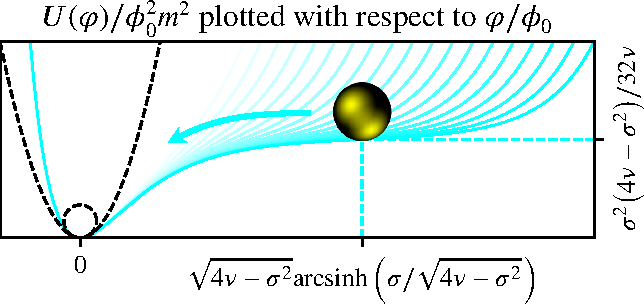
\includegraphics[width=1\linewidth]{Inflaton.pdf}
	 \caption{Massive scalar perturbations in~\cref{EinsteinKleinGordon} have a unique, non-linear, scale-invariant embedding given in~\cref{ToyModel}. This embedding can lead to only one qualitative alteration in~\cref{FullTheory,Potential}: the quadratic potential (dashed, with a unit-circle illustrating the mass scale~$m$) develops a non-linear plateau (cyan) whose depth and height depend on model parameters~$\nu$ and~$\sigma$. The plateau is consistent with current CMB constraints on a slowly-rolling inflaton (arrow).}
 	\label{PotentialFig}
 \end{figure}

\paragraph*{Scale-invariant embedding} For our toy model, we work just with the matter sector. Let us suppose we know that some scalar perturbations~$\delta\varphi$ have a Klein--Gordon mass~$m$ 
\begin{equation}\label{EinsteinKleinGordon}
	S=\int\mathrm{d}^4x\sqrt{-g}\left[\tfrac{1}{2}\PD{_\mu}\delta\varphi\ \PD{^\mu}\delta\varphi-\tfrac{1}{2}m^2\delta\varphi^2+\text{gravity}\right],
\end{equation}
where we allow the theory to be minimally coupled to a metric-based gravity theory (e.g. GR). This situation already arises in cosmology: we typically infer that the canonical inflaton potential is approximated by a mass term~$U(\varphi)=m^2\varphi^2/2+\dots$ in order to facilitate reheating into the SM plasma after the end of inflation\footnote{Strictly, this is only true for `textbook' slow-roll inflation~\cite{Hobson:2006se,Vazquez:2018qdg,Achucarro:2022qrl}. We particularly note that Higgs inflation does not require a reheating mass~\cite{Bezrukov:2007ep}.}~\cite{Allahverdi:2010xz}. This inference does not, however, place constraints on~$U(\varphi)$ beyond the~$\delta\varphi$ linear regime. For a host of reasons the most favoured non-linear completion envisages~$\varphi$ rolling off a plateau in~$U(\varphi)$ sufficiently slowly to drive~$N\sim 55$ e-folds of inflation~\cite{Planck:2013jfk,Planck:2015sxf,Planck:2018jri}. Quite how this plateau should be motivated through fundamental theory is not yet settled. What we want to show here is that, starting purely from the linear model in~\cref{EinsteinKleinGordon}, there is a way to build up the non-linear plateau by asking that~$m$ be a dynamically acquired mass scale in a locally scale-invariant `embedding' theory (see~\cref{PotentialFig}). There is precedent here, since~\cref{EinsteinKleinGordon} also describes pions~\cite{Georgi:1984zwz,Donoghue:1992dd,Manohar:2000dt,Scherer:2012xha}. Pion masses, however, emerge long after reheating, through chiral and electroweak symmetry breaking~\cite{Higgs:1964pj,Guralnik:1964eu}. Moreover, the absence of explicit mass scales only makes the SM \emph{globally} scale-invariant. Under \emph{local} rescalings, the metric deforms as~$\FieldG{_{\mu\nu}}\mapsto e^{2\rho}\FieldG{_{\mu\nu}}$ and the scalar as~$\varphi\mapsto e^{-\rho}\varphi$ for local~$\rho\equiv\rho(x)$. Considering the first term in~\cref{EinsteinKleinGordon}, we must therefore introduce a \emph{Weyl} vector~$\FieldV{_\mu}\mapsto\FieldV{_\mu}-\PD{_\mu}\rho$ to define a new covariant derivative on scalars~$\SCovD{_\mu}\varphi\equiv\big(\PD{_\mu}-\FieldV{_\mu}\big)\varphi$. The kinematic d.o.f are thus increased from~$\big\{\FieldG{_{\mu\nu}},\varphi\big\}$ to~$\big\{\FieldG{_{\mu\nu}},\varphi,\FieldV{_\mu}\big\}$. Next, considering the second term in~\cref{EinsteinKleinGordon}, we must introduce a \emph{compensator} scalar~$\phi\mapsto e^{-\rho}\phi$ to make up the mass dimension of~$m$, which now becomes a dimensionless parameter. In the effective field theory approach, the non-linear completion of~\cref{EinsteinKleinGordon} includes all scale-invariant operators of mass-dimension four in the new variables~$\big\{\FieldG{_{\mu\nu}},\varphi,\FieldV{_\mu},\phi\big\}$, namely
\begin{align}\label{ToyModel}
		S=\int\mathrm{d}^4x\sqrt{-g}\Big[&\frac{1}{2}\SCovD{_\mu}\varphi\SCovD{^\mu}\varphi
		-\frac{\sigma}{2}\SCovD{_\mu}\varphi\SCovD{^\mu}\phi
		+\frac{\nu}{2}\SCovD{_\mu}\phi\SCovD{^\mu}\phi
		\nonumber\\&
		\hspace{-25pt}
		-\frac{\mu^2}{2}\phi^2\varphi^2
		-\frac{\xi}{16}\MAGH{_{\mu\nu}}\MAGH{^{\mu\nu}}+\text{gravity}\Big],
\end{align}
where~$\mu$,~$\sigma$,~$\nu$ and~$\xi$ are dimensionless model parameters, and~$\MAGH{_{\mu\nu}}\equiv 2\PD{_{[\mu}}\FieldV{_{\nu]}}$ is the natural Weyl field-strength tensor, i.e.~$\SCovD{_{[\mu}}\SCovD{_{\nu]}}\varphi\equiv-\frac{1}{2}\MAGH{_{\mu\nu}}\varphi$. For brevity we omit the~$\varphi^4$ and~$\phi^4$ self-interaction terms, though we still expect inflation to be a viable outcome with these terms present.\footnote{We will find that the~$\varphi^4$ operator deforms the potential without (visually) compromising the desired slow-roll plateau, though a detailed comparison with the CMB is lacking; the~$\phi^4$ operator provides a cosmological constant, which can be neglected when considering the early-Universe physics.}

\paragraph*{Scale-invariant variables} One can compare~$\FieldV{_\mu}$ to the electromagnetic four-vector potential. But unlike in scalar electrodynamics, where the matter fields carry a non-physical phase as well as a physical magnitude, the fields~$\varphi$ and~$\phi$ each have only one real d.o.f which merges entirely with the choice of scale gauge. This means that the field equations of~\cref{ToyModel} cannot simultaneously propagate~$\varphi$ and~$\phi$ from the initial data:\footnote{The scale-invariance of this model is local, i.e. it constitutes a gauge symmetry. To propagate the fields in the presence of a gauge symmetry, not only must the initial data be specified at some time-slice, but also the choice of gauge (in our case, the value of~$\phi$) at all future times must be agreed upon~\cite{Henneaux:1992ig}. The same scenario arises in classical electromagnetism and in GR: it does not detract from the well-posedness of the model.} we must first declare a global solution for one of these fields. Remembering that we want to recover~\cref{EinsteinKleinGordon}, we may take the opportunity to eliminate~$\phi$ by assuming constant~$\phi=\phi_0$. This is the \emph{Einstein} choice of scale gauge. Rather than imposing the Einstein gauge, it is instead possible to eliminate~$\phi$ completely from~\cref{ToyModel} through the field reparameterisations~$\FieldG{_{\mu\nu}}\mapsto(\phi_0/\phi)^2\FieldGHat{_{\mu\nu}}$, $\varphi\mapsto\phi\hat\varphi/\phi_0$ and~$\FieldV{_\mu}\mapsto\FieldVHat{_\mu}+\PD{_\mu}\ln\phi$, resulting in
\begin{align}\label{ScaleInvariantVariables}
	S=\int\mathrm{d}^4x\sqrt{-\hat g}\Big[&\frac{1}{2}\left(\PD{_\mu}\hat\varphi-\left(\hat\varphi-\sigma\phi_0\right)\FieldVHat{_\mu}\right)\left(\PD{^\mu}\hat\varphi-\hat\varphi\FieldVHat{^\mu}\right)
		\nonumber\\&
		\hspace{-60pt}
		-\frac{\mu^2\phi_0^2}{2}\hat\varphi^2
		-\frac{\xi}{16}\MAGHHat{_{\mu\nu}}\MAGHHat{^{\mu\nu}}
		+\frac{\nu\phi_0^2}{2}\FieldVHat{_\mu}\FieldVHat{^\mu}
		+\text{gravity}\Big],
\end{align}
where we note~$\MAGHHat{_{\mu\nu}} \equiv 2\PD{_{[\mu}}\FieldVHat{_{\nu]}}\equiv 2\PD{_{[\mu}}\FieldV{_{\nu]}}\equiv \MAGH{_{\mu\nu}}$. By construction, the new fields~$\big\{\FieldGHat{_{\mu\nu}},\hat\varphi,\FieldVHat{_\mu}\big\}$ are \emph{scale-invariant variables}. The gauge symmetry in~\cref{ScaleInvariantVariables} seems to be destroyed, but we now understand that the rescaling transformations are still happening internally within the new fields. Scale-invariant variables and the Einstein gauge choice both result in~\cref{ScaleInvariantVariables}, a key feature of which is that the dimensionless couplings are now accompanied by powers of~$\phi_0$. We will return to the natural values of these couplings later.

\paragraph*{Bootstrapping inflation} After dropping the hats, shifting the vector by the scalar gradient to remove the cross-term and rescaling both fields\footnote{Note during the rescaling~$\FieldV{_\mu}\mapsto\FieldV{_\mu}/\sqrt{\xi}$ that unitarity requires~$\xi\geq 0$.}, and for perturbations~$\delta\varphi$ and~$\delta\FieldV{_\mu}$ around the vacuum~$\varphi=\FieldV{_\mu}= 0$, we find that~\cref{ScaleInvariantVariables} reduces to
\begin{align}\label{PerturbativeTheory}
S&=\int\mathrm{d}^4x\sqrt{-g}\Big[\frac{1}{2}\PD{_\mu}\delta\varphi\PD{^\mu}\delta\varphi-\frac{m^2}{2}\delta\varphi^2\nonumber\\
	&-\frac{1}{4}\PD{_{[\mu}}\delta\FieldV{_{\nu]}}\PD{^{[\mu}}\delta\FieldV{^{\nu]}}+\frac{M^2}{2} \delta\FieldV{_\mu}\delta\FieldV{^\mu}+\text{gravity}\Big],
\end{align}
where~$m^2\equiv4\nu\mu^2\phi_0^2/(4\nu-\sigma^2)$ and~$M^2\equiv\nu\phi_0^2/\xi$. This result is very interesting. Not only do we recover~\cref{EinsteinKleinGordon} in the first line of~\cref{PerturbativeTheory}, but we see how local scale invariance additionally points to the presence of a new Proca field. To compare, the Higgs mechanism pointed to the presence of a new massive scalar, which was later observed experimentally~\cite{CMS:2012qbp}. Arguably, there is no need for a new vector in particle physics or cosmology. But whilst~$\nu\to 0$ predicts two radiative d.o.f which are not observed, taking instead~$\nu\to \infty$ nonetheless gives a heavy-enough Proca to evade all observational bounds (even better, it may be a dark matter candidate~\cite{Lasenby:2015dba}). Beyond the perturbative regime, the Proca and Klein--Gordon fields acquire non-linear interactions. For sufficiently large~$\nu$ the Proca can be eliminated as~$\FieldV{_\mu}=\frac{1}{2}\PD{_\mu}\ln\left(\varphi^2-\sigma\phi_0\varphi+\nu\phi_0^2\right)$ on-shell,\footnote{A specific regime is~$\nu\gg\sigma^2$ where the gauge boson is weakly coupled by~$\xi\gtrsim 1$. We work in Planck units, assuming Weyl symmetry breaking at~$\phi_0\sim\MPl{}$. An effective scalar theory emerges at~$\mu^2\ll\mathcal{E}^2\ll\nu/\xi$ from which we retain only the zeroth-order correction in the~$\mathcal{E}^2/M^2$ expansion to reach~\cref{FullTheory,Potential}. A visual comparison between~\cref{PotentialFig} and the potential in~\cite{Salvio:2022suk} suggests agreement with the CMB when the field value at slow roll is~$\sigma\sim 10$ and the scale of inflation is~$\sigma^2\mu^2\sim 10^{-10}$. This yields an inflaton of mass~$\mu\sim 10^{-6}$ or~$m\sim 10^{13}\SI{}{\giga\electronvolt}$. Meanwhile, the vector mass~$M$ approaches the Planck scale for stronger couplings at smaller~$\xi$.} and~\cref{ScaleInvariantVariables} becomes
\begin{subequations}
\begin{align}
	&S=\int\mathrm{d}^4x\sqrt{-g}\left[\tfrac{1}{2}\PD{_\mu}\varphi\PD{^\mu}\varphi-U\left(\varphi\right)+\text{gravity}\right],\label{FullTheory}\\
	&U\left(\varphi\right)\equiv\frac{\mu^2\phi_0^4}{2}\left[\frac{\sigma}{2}+\sqrt{\nu-\frac{\sigma^2}{4}}\text{sinh}\left(\frac{(\varphi-c)/\phi_0}{\sqrt{\nu-\frac{\sigma^2}{4}}}\right)\right]^{\ 2},\label{Potential}
\end{align}
\end{subequations}
where~$c$ is an integration constant.\footnote{Note that the scalar in~\cref{FullTheory,Potential} has been recanonicalised, so that all the physical implications may be read off from the potential~$U$. If a~$\varphi^4$ operator had been included in~\cref{ToyModel}, then~\cref{FullTheory} would feature an additional~$U^2$ operator. In this case, model parameters may still be found which reproduce the plateau associated with slow-roll inflation; we are not, however, aware of any CMB constraints on this extended model.} The non-linear potential (see~\cref{PotentialFig}) is identical to that found in~\cite{Barker:2024dhb,Salvio:2022suk}, though the motivations are unrelated. The predictions from the inflationary plateau approach the universal values for the spectral index~$n_s\approx 1-2/N$ and also the tensor-to-scalar ratio~$r\approx12/N^2$ for appropriate values of the model parameters~\cite{Salvio:2022suk,Karananas:2025xcv}.\footnote{It remains to be investigated, however, whether the universal regime is consistent with a weakly-coupled gauge boson.} This agrees with current cosmic microwave background (CMB) measurements~\cite{Planck:2018jri,BICEP:2021xfz}, pending future experiments~\cite{arXiv:1110.3193,Weltman:2018zrl,Abazajian:2019eic,LiteBIRD:2022cnt}. The inverse problem of constraining (through Bayesian inference) the model parameters from the CMB observations is well within the scope of precision cosmology~\cite{Handley:2019fll}. We will develop this toy model in future work, but first need to make the `$+\ \text{gravity}$' term more concrete.

\paragraph*{Recap and extension} Collecting our results so far:
\begin{enumerate}
	\item Gravitational coupling to fermions naturally leads to PGT as a leading formulation of gravity. PGT does not have local scale invariance.
	\item The~$\PD{_{[\mu}}\MAGT{_{\nu]}}\PD{^{[\mu}}\MAGT{^{\nu]}}$ term for vector torsion~$\MAGT{_\mu}$ is notoriously absent from the PGT action in~\cref{PGTAction}.
	\item Theories with mass scales have locally-scale-invariant embeddings which can lead to excellent phenomenology (inflation) besides a new massive vector~$\FieldV{_\mu}$.
\end{enumerate}
We will now connect these three observations by showing that eWGT is the unique scale-invariant embedding of PGT. This will identify~$\MAGT{_\mu}/3$ with the vector~$\FieldV{_\mu}$ when expressed in scale-invariant variables, and thereby reveal~$\PD{_{[\mu}}\MAGT{_{\nu]}}\PD{^{[\mu}}\MAGT{^{\nu]}}$ to be a Yang--Mills-type term.

\paragraph*{Poincar\'e gauge theory (PGT)} Gauge theories of gravity can be formulated on completely flat Minkowski spacetime, just like the SM~\cite{Lasenby:2015dba}. In this formulation, we use holonomic Greek indices and Lorentz Roman indices. Translational gauge fields~$\FieldB{^i_\mu}$ and inverses~$\FieldH{_i^\mu}$ obey~$\FieldB{^i_\mu}\FieldH{_i^\nu}\equiv\FieldDelta{_\mu^\nu}$ and~$\FieldB{^i_\mu}\FieldH{_j^\mu}\equiv\FieldDelta{_j^i}$, and give rise to the curved-space metric~$\FieldG{_{\mu\nu}}$ through~$\FieldB{^i_\mu}\FieldB{^j_\nu}\FieldEta{_{ij}}\equiv\FieldG{_{\mu\nu}}$. We assume contraction with these fields eliminates all coordinate indices of general (i.e. not necessarily scalar) matter fields~$\varphi$, which have only suppressed Lorentz (or spinor) indices. A general~$\varphi$ with Weyl weight~$w$ and belonging to the~$\mathrm{SL}(2,\mathbb{C})$ representation with Lorentz generators~$\FieldSigma{_{ij}}\equiv\FieldSigma{_{[ij]}}$ transforms as~$\varphi\mapsto e^{w\rho+\FieldOmega{^{ij}}\FieldSigma{_{ij}}/2}\varphi$, where~$\FieldOmega{^{ij}}\equiv\FieldOmega{^{[ij]}}(x)$ are finite angles. The rotational gauge field is~$\FieldA{^{ij}_\mu}\equiv\FieldA{^{[ij]}_\mu}$. The transformations~$\FieldB{^i_\mu}\mapsto e^{\rho}\FieldLambda{^i_j}\FieldB{^j_\mu}$ and~$\FieldA{^{ij}_\mu}\mapsto\FieldLambda{^i_k}\FieldLambda{^j_l}\FieldA{^{kl}_\mu}-\FieldLambda{^{jk}}\PD{_\mu}\FieldLambda{^i_k}$ (where~$\FieldLambda{}\equiv e^{\FieldOmega{}}$ is the Lorentz matrix) ensure that the derivative~$\SCovD{_i}\equiv\FieldH{_i^\mu}\SCovD{_\mu}$ with
\begin{equation}\label{PGTDer}
\SCovD{_\mu}\varphi\equiv\left(\PD{_\mu}+\tfrac{1}{2}\FieldA{^{ij}_\mu}\FieldSigma{_{ij}}\right)\varphi,
\end{equation}
is Lorentz-covariant. The field strengths from the commutator~$\FieldB{^{[i|}_\mu}\FieldB{^{|j]}_\nu}\SCovD{_{[i}}\SCovD{_{j]}}\varphi\equiv\frac{1}{4}\FieldB{^{i}_\sigma}\FieldB{^j_\lambda}\MAGF{^{\sigma\lambda}_{\mu\nu}}\FieldSigma{_{ij}}\varphi-\frac{1}{2}\MAGT{^\lambda_{\mu\nu}}\SCovD{_\lambda}\varphi$ are
\begin{subequations}
\begin{align}	\MAGT{^\lambda_{\mu\nu}}&\equiv2\FieldH{_i^\lambda}(\PD{_{[\mu|}}\FieldB{^i_{|\nu]}}+\FieldA{^i_j_{[\mu|}}\FieldB{^j_{|\nu]}}),\label{Torsion}\\
\MAGF{^{\rho\sigma}_{\mu\nu}}&\equiv2\FieldH{_i^\rho}\FieldH{_j^\sigma}(\PD{_{[\mu|}}\FieldA{^{ij}_{|\nu]}}+\FieldA{^i_k_{[\mu|}}\FieldA{^{kj}_{|\nu]}}),\label{Curvature}
\end{align}
\end{subequations}
where~\cref{Torsion,Curvature} are equivalent to~\cref{ECTorsion,ECCurvature}; the reparameterisation from gauge-theoretic~$\big\{\FieldB{^i_\mu},\FieldA{^{ij}_\mu}\big\}$ to geometric~$\big\{\FieldG{_{\mu\nu}},\MAGA{^\alpha_{\mu}_{\nu}}\big\}$ is described in~\cite{Blagojevic:2002,Lasenby:2015dba}.

\paragraph*{Weyl gauge theory (WGT)} From our toy model, the Weyl-covariant extension of~\cref{PGTDer} is 
\begin{equation}\label{WGTDer}
\SCovD{_\mu}\varphi\equiv\left(\PD{_\mu}+\tfrac{1}{2}\FieldA{^{ij}_\mu}\FieldSigma{_{ij}}+w\FieldV{_\mu}\right)\varphi,
\end{equation}
and this construction defines the well-known \emph{Weyl gauge theory} (WGT) of gravity~\cite{Weyl:1918ib,Weyl:1931}. Whilst~$\MAGF{^{\rho\sigma}_{\mu\nu}}$ in~\cref{Curvature} is already Weyl-covariant, we have under local dilations
\begin{equation}\label{TorsionTransform}
	\MAGT{^\lambda_{\mu\nu}}\mapsto \MAGT{^\lambda_{\mu\nu}}-2\FieldDelta{^\lambda_{[\mu}}\PD{_{\nu]}}\rho\implies\MAGT{_\mu}\mapsto\MAGT{_\mu}-3\PD{_\mu}\rho,
\end{equation}
so from~\cref{TorsionTransform} only the combination
\begin{equation}\label{TracelessTorsion}
\MAGTTilde{^\lambda_{\mu\nu}}\equiv\MAGT{^\lambda_{\mu\nu}}-2\FieldDelta{^\lambda_{[\mu}}\FieldV{_{\nu]}},
\end{equation}
is covariant, indeed~$\FieldB{^{[i|}_\mu}\FieldB{^{|j]}_\nu}\SCovD{_{[i}}\SCovD{_{j]}}\varphi\equiv\frac{1}{4}\FieldB{^{i}_\sigma}\FieldB{^j_\lambda}\MAGF{^{\sigma\lambda}_{\mu\nu}}\FieldSigma{_{ij}}\varphi-\frac{1}{2}\MAGTTilde{^\lambda_{\mu\nu}}\SCovD{_\lambda}\varphi+\frac{1}{2}w\MAGH{_{\mu\nu}}\varphi$. Following~\cref{ToyModel}, the parity-even Yang--Mills-type embedding of~\cref{PGTAction} must then be strictly
\begin{align}\label{WGTAction}
	&S_{\text{WGT}}\equiv\int\mathrm{d}^4x\sqrt{-g}\Big[
	-\frac{\zeta\phi^2}{2}\MAGF{}
	-\lambda\phi^4
	+\Alp{1}\MAGF{}^2
	+\MAGF{_{\mu\nu}}\big(
	\Alp{2}\MAGF{^{\mu\nu}}
	\nonumber\\ &
	+\Alp{3}\MAGF{^{\nu\mu}}\big)
	+\MAGF{_{\mu\nu\sigma\lambda}}\big(
	\Alp{4}\MAGF{^{\mu\nu\sigma\lambda}}
	+\Alp{5}\MAGF{^{\mu\sigma\nu\lambda}}
	+\Alp{6}\MAGF{^{\sigma\lambda\mu\nu}}\big)
	\nonumber\\ &
	+\phi^2\MAGTTilde{_{\mu\nu\sigma}}\big(\Gam{1}\MAGTTilde{^{\mu\nu\sigma}}
	+\Gam{2}\MAGTTilde{^{\nu\mu\sigma}}\big)
	+\phi^2\Gam{3}\MAGTTilde{_{\mu}}\MAGTTilde{^{\mu}}
	+\frac{\nu}{2}\SCovD{_\mu}\phi\SCovD{^\mu}\phi
	\nonumber\\ &
	-\frac{\xi}{16}\MAGH{_{\mu\nu}}\MAGH{^{\mu\nu}}
	+\frac{\chi}{2}\MAGF{_{\mu\nu}}\MAGH{^{\mu\nu}}
	+\text{matter}
	\Big],
\end{align}
with dimensionless~$\zeta$,~$\lambda$,~$\Gam{1}$,~$\Gam{2}$,~$\Gam{3}$,~$\nu$,~$\xi$,~$\chi$ and~$\alpha_1$ through~$\alpha_6$. Crucially, everything is quadratic in field strengths.

\paragraph*{Extended Weyl gauge theory (eWGT)} In moving from PGT to WGT, we have enlarged the kinematic space from~$\big\{\FieldB{^i_\mu},\FieldA{^{ij}_\mu}\big\}$ to~$\big\{\FieldB{^i_\mu},\FieldA{^{ij}_\mu},\FieldV{_\mu},\phi\big\}$, just like in our toy model. Unlike for our toy model, however, the enlargement proves unnecessary: it is more economical to recycle~$\FieldV{_\mu}$ from within the rotational gauge field. Let the traceless part of the latter field be~$\FieldATilde{^{ij}_{\mu}}\equiv\FieldATilde{^{[ij]}_{\mu}}$ with only 20 d.o.f, such that~$\FieldH{_j^\nu}\FieldATilde{^{ij}_\nu}\equiv 0$. Then, using~$\big\{\FieldB{^i_\mu},\FieldATilde{^{ij}_\mu},\FieldV{_\mu},\phi\big\}$ there is one (and \emph{only} one) way to emulate the combined Poincar\'e and Weyl covariance of~\cref{WGTDer}, namely
\begin{align}
	\SCovD{_\mu}\varphi\equiv\Big(\PD{_\mu}+\tfrac{1}{2}\Big[&\FieldATilde{^{ij}_\mu}-\tfrac{2}{3}\FieldB{^{[i|}_\mu}\FieldH{^{|j]}^\nu}\big(3\FieldV{_\nu}
	\nonumber\\&\ \ \ 
	-2\FieldH{_k^\lambda}\PD{_{[\lambda|}}\FieldB{^k_{|\nu]}}\big)\Big]\Sigma{_{ij}}+w\FieldV{_\mu}\Big)\varphi.\label{EconomicalAction}
\end{align}
Although unique,\footnote{The extra terms in the square brackets in~\cref{EconomicalAction} have been constructed so as to emulate the inhomogeneous Lorentz transformation of the (missing) trace vector~$\FieldH{_j^\nu}\FieldA{^{ij}_\nu}$, without simultaneously generating an (unwanted) inhomogeneous Weyl transformation. There is only one such construction. One might ask whether a similar trick can be used to replace the axial vector~$\tensor{\epsilon}{^k_{ijl}}\FieldH{_k^\nu}\FieldA{^{ij}_\nu}$. The answer is of course affirmative, but the construction in this case does not need (and must not contain)~$\FieldV{_\mu}$ because the axial vector and purely tensor parts of the Ricci rotation coefficients are already Weyl-covariant: only the trace vector part has an inhomogeneous Weyl transformation, which requires correcting via~$\FieldV{_\mu}$ in the manner proposed. By carefully propagating this observation through to our main result in~\cref{eWGTAction}, we conclude that local scale invariance always leads to dynamical \emph{vector} torsion, and not \emph{axial vector} torsion.}we will soon show that~\cref{EconomicalAction} is just one notational way to write the eWGT covariant derivative from~\cite{Lasenby:2015dba}. Because eWGT shares the symmetries of WGT, it must also share the Yang--Mills-type action in~\cref{WGTAction}. The difference is that we must replace~$\FieldA{^{ij}_\mu}$, as when going from~\cref{WGTDer} to~\cref{EconomicalAction}. After this change, we notice from~\cref{TracelessTorsion} that~$\MAGTTilde{_\mu}\equiv 0$ identically. Thus,~$\Gam{3}$ in~\cref{WGTAction} drops out of eWGT.

\paragraph*{Equivalence of PGT and eWGT} With the field reparameterisation~$\FieldV{_\mu}\mapsto\FieldVV{_\mu}+\frac{2}{3}\FieldH{_k^\lambda}\PD{_{[\lambda|}}\FieldB{^k_{|\mu]}}$ we find~\cref{EconomicalAction} is 
\begin{align}
	\SCovD{_\mu}\varphi\equiv\Big(\PD{_\mu}+\tfrac{1}{2}\Big[&\FieldATilde{^{ij}_\mu}-2\FieldB{^{[i|}_\mu}\FieldH{^{|j]}^\nu}\FieldVV{_\nu}\Big]\Sigma{_{ij}}
	\nonumber\\&\ \ \ 
	+w\Big[\FieldVV{_\mu}+\tfrac{2}{3}\FieldH{_k^\lambda}\PD{_{[\lambda|}}\FieldB{^k_{|\mu]}}\Big]\Big)\varphi.\label{TrimmedAction}
\end{align}
In this~$\big\{\FieldB{^i_\mu},\FieldATilde{^{ij}_\mu},\FieldVV{_\mu},\phi\big\}$ formulation~$\FieldVV{_\mu}$ is a `Lorentz' boson, not a `Weyl' boson, because~$\FieldVV{_\mu}\mapsto\FieldVV{_\mu}-\frac{1}{3}\FieldH{^\lambda_l}\FieldB{^m_\mu}\FieldLambda{_k^l}\PD{_\lambda}\FieldLambda{^k_m}$. Relabelling~$\FieldA{^{ij}_\mu}\equiv\FieldATilde{^{ij}_\mu}-2\FieldB{^{[i|}_\mu}\FieldH{^{|j]}^\nu}\FieldVV{_\nu}$, where~$\FieldA{^{ij}_\mu}\equiv\FieldA{^{[ij]}_\mu}$ carries 24 d.o.f, ensures the PGT transformation of~$\FieldA{^{ij}_\mu}$. In this~$\big\{\FieldB{^i_\mu},\FieldA{^{ij}_\mu},\phi\big\}$ formulation~\cref{TrimmedAction} becomes
\begin{align}
	\SCovD{_\mu}\varphi&\equiv\Big(\PD{_\mu}+\tfrac{1}{2}\FieldA{^{ij}_\mu}\Sigma{_{ij}}
	+\tfrac{1}{3}w\FieldH{_k^\lambda}\Big[2\PD{_{[\lambda|}}\FieldB{^k_{|\mu]}}+3\FieldB{_l_\mu}\FieldA{^{kl}_\lambda}\Big]\Big)\varphi
	\nonumber\\&
	\equiv\Big(\PD{_\mu}+\tfrac{1}{2}\FieldA{^{ij}_\mu}\Sigma{_{ij}}
	+\tfrac{1}{3}w\MAGT{_\mu}\Big)\varphi,
\label{PreAction}
\end{align}
where we used~\cref{Torsion} in the last equality. New fields should not be introduced where they are not needed: in hindsight it was obvious from~\cref{TorsionTransform} that PGT contained a vector~$\MAGT{_\mu}/3$ which already performed the function of~$\FieldV{_\mu}$. This fact was observed by Obukhov in~\cite{Obukhov:1982zn}, and the covariant derivative in~\cref{PreAction} was first written down in~\cite{Lasenby:2015dba} (see also~\cite{Karananas:2021gco}). One could interpret~\cref{PreAction} as a hint that PGT descends from a scale-invariant theory. Explicit scales emerge in the~$\big\{\FieldBHat{^i_\mu},\FieldAHat{^{ij}_\mu}\big\}$ formulation, with scale-invariant variables~$\FieldB{^i_\mu}\mapsto\phi_0\FieldBHat{^i_\mu}/\phi$ and~$\FieldA{^{ij}_\mu}\mapsto\FieldAHat{^{ij}_\mu}$. By dropping the hats on variables, we find that the PGT Lagrangian couplings parameterise exactly the same physics as the following combinations of eWGT couplings (with  $\alpha_1,\ldots,\alpha_6$ identical)
\begin{equation}\label{Equivalences}
	\begin{gathered}
		\MPl{}^2\equiv \zeta\phi_0^2,\quad \MPl{}^2\Lambda\equiv\lambda\phi_0^4,\quad \Bet{1}\equiv\Gam{1}\phi_0^2,\\
		\Bet{2}\equiv\Gam{2}\phi_0^2,\quad \Bet{3}\equiv\big(\nu-6(2\Gam{1}+\Gam{2})\big)\phi_0^2/18.
	\end{gathered}
\end{equation}
Although the~$\Gam{3}$ coupling of WGT in~\cref{WGTAction} is missing from the eWGT action, its loss is exactly compensated for by~$\nu$ so that~$\Bet{3}$ emerges in~\cref{Equivalences} as an independent coupling in PGT. The couplings~$\chi$ and~$\xi$ do not appear in~\cref{Equivalences} --- these parameterise terms involving~$\MAGH{_{\mu\nu}}$, which is the Faraday tensor for~$\MAGT{_\mu}$ in the scale-invariant variables of PGT. Thus, eWGT motivates a correction to Yang--Mills-type PGT:
\begin{align}\label{eWGTAction}
	S_{\text{eWGT}}\equiv S_{\text{PGT}}
	+\frac{1}{3}\int\mathrm{d}^4x\sqrt{-g}\Big[&
	\chi\MAGF{_{[\mu\nu]}}\PD{^{[\mu}}\MAGT{^{\nu]}}
	\nonumber\\&
	-\frac{\xi}{12}\PD{_{[\mu}}\MAGT{_{\nu]}}\PD{^{[\mu}}\MAGT{^{\nu]}}
	\Big].
\end{align}
This is our central result: the relationship between~\cref{eWGTAction} and~\cref{PGTAction} is analogous to the relationship between~\cref{FullTheory} and~\cref{EinsteinKleinGordon}. Put another way, the traditional PGT action unfairly omits two specific terms, which are naturally motivated by the unique, scale-invariant embedding. This embedding allows us to claim that all PGT models are ultimately conformal, irrespective of the explicit mass scales in their spectra. We confirm in the supplemental material~\cite{Barker:2024} that eWGT, as formulated in~\cref{TracelessTorsion,WGTAction,EconomicalAction}, and the extension of PGT in~\cref{eWGTAction,PGTAction,Torsion,Curvature}, have completely equivalent spectra. In the expressions for masses and pole residues,~\cref{Equivalences} maps the dimensionful couplings to their dimensionless counterparts.\footnote{As a final remark, we return to the values of the dimensionless couplings. If one retains the forms of the coefficients on the RHS of~\cref{Equivalences} in the eWGT action, it is natural first to pull out a constant factor of $\phi_0^2$, which has the same dimensions as $\MPl{}^2$. 
When concerned with physics at the length-scale~$\LPhy{}$, it is helpful to work in units of~$\LPhy{}$. This can be done by taking~$\phi_0\LPhy{}\equiv 1$ as a gauge choice in the remainder of the action, which is equivalent to the standard practice of setting $\phi_0 = 1$ provided one works in length units of $\LPhy{}$. If one instead works in some other length units of $\LPhyprime{}$, then one should rescale $\phi_0$ by $\LPhyprime{}/\LPhy{}$. Having set $\phi_0=1$, however, it is the dimensionless couplings that should `run' with the length units used. This `running' is intended in a more prosaic sense than the action of beta functions in the quantum theory. Any classical field equations can, in some system of units, be integrated from a fixed numerical range of initial data and for a fixed numerical interval. The resulting solutions may look very different, depending on the numerical values of the couplings in the equations. These different solutions describe phenomena on different physical scales, and the values of the couplings are tied to these scales. To give a concrete example, the mass in the Klein--Gordon equation can be neglected numerically when the dynamics are probed at distances much shorter than the Compton wavelength. In our case, by observing the powers of $\phi_0$ associated with each dimensionless coupling constant (after factorising out $\phi^2_0$ as discussed above), it is straightforward to show that $\zeta$, $\nu$, and the $\beta$s do not change with scale (and so presumably should have values $\sim 1$), whereas the $\alpha$s, $\xi$ and $\chi$ scale as $(\LPhyprime{}/\LPhy{})^{-2}$, while $\lambda$ scales as $(\LPhyprime{}/\LPhy{})^2$. On adopting the convention~$\LPl{}\MPl{}\equiv 1$, it is worth noting from~\cref{Equivalences} that $\lambda\sim\SI{1e-122}{}(\LPhy{}/{\LPl{}})^2 \sim 1$ at the scale~$\LPhy{}\sim\SI{10}{\giga\parsec}$, which is close to the Hubble horizon.}

\paragraph*{Implications for the PGT spectrum} Since we have made a substantial correction to the PGT Lagrangian, it is important to update the well-known PGT particle spectrum in~\cite{Hayashi:1980qp}. To do this, we take~$\lambda= \Lambda = 0$ and focus on the linearisation near Minkowski spacetime. As shown in~\cref{ParticleSpectra} and~\cref{ParticleSpectrographGeneralCase}, the propagator of~$S_{\text{eWGT}}$ in~\cref{eWGTAction} contains a \emph{quartic} pole in the parity-odd spin-one sector
\begin{align}
	\label{MasterConstraint}
	&2\Big[\big(2\Alp{2}+4\Alp{4}+\Alp{5}\big)\xi-\chi^2\Big]k^4
	+3\Big[
		96\Alp{2}\big(2\Bet{1}+\Bet{2}+\Bet{3}\big)
		\nonumber\\&
		+8\big[24\Alp{4}\big(2\Bet{1}+\Bet{2}+\Bet{3}\big)+6\Alp{5}\big(2\Bet{1}+\Bet{2}+\Bet{3}\big)
		\nonumber\\&
		+\chi\big(4\Bet{1}+2\Bet{2}-\MPl{}^2\big)\big]+\big(4\Bet{1}+2\Bet{2}-\MPl{}^2\big)\xi
	\Big]k^2
		\nonumber\\&
	+72\big(4\Bet{1}+2\Bet{2}-\MPl{}^2\big)\big(2\Bet{1}+\Bet{2}+3\Bet{3}+\MPl{}^2\big).
\end{align}
The pole takes the familiar~$k^2-M^2$ form when the~$k^4$ coefficient is removed from~\cref{MasterConstraint}. For example, the branch~$2\Alp{2}+4\Alp{4}+\Alp{5}=\chi=0$ contains the Einstein--Proca theory (EPT)~$S_{\text{EPT}}\equiv\int\mathrm{d}^4x\sqrt{-g}\big[-\frac{1}{2}\MPl{}^2\rR{}-\frac{1}{4}\PD{_{[\mu}}\MAGT{_{\nu]}}\PD{^{[\mu}}\MAGT{^{\nu]}}+\frac{1}{2}M^2\MAGT{_\mu}\MAGT{^\mu}+\text{matter}\big]$ in~$\big\{\FieldG{_{\mu\nu}},\MAGT{^\alpha_{\mu}_{\nu}}\big\}$ variables. EPT is evidently not strongly coupled, so this is the much-sought-after \emph{vector torsion}. The more general branch~$\Alp{5}=\chi^2/\xi-2\left(\Alp{2}+2\Alp{4}\right)$ leads to the new mass spectrum in~\crefrange{Mass0p}{Mass2m}, as shown in~\cref{ParticleSpectrographGeneralCaseNoQuartic}. It is also interesting to instead remove the \emph{constant} term in~\cref{MasterConstraint}. This produces a~$k^2\big(k^2-M^2\big)$ pole, which affects the massless spectrum. As shown in~\cref{ParticleSpectrographBranch1Conservative}, we find an example case~$\Alp{2}=\Alp{3}-4\Alp{4}+\Alp{6}=4\Alp{4}+\Alp{5}=4\Bet{1}+2\Bet{2}-\MPl{}^2=0$ which propagates (without ghosts or tachyons) the Einstein graviton, one heavy scalar, one heavy pseudoscalar, and a \emph{one extra massless scalar}. To understand where this scalar comes from, we strip away all the uninvolved operators to show in~\cref{ParticleSpectrographSwitchonPGT} that the model 
\begin{equation}\label{SwitchonPGT}
	S=\int\mathrm{d}^4x\sqrt{-g}\big[\chi\MAGF{_{[\mu\nu]}}\PD{^{[\mu}}\MAGT{^{\nu]}}+\Bet{3}\MAGT{_{\mu}}\MAGT{^{\mu}}\big],	
\end{equation}
propagates, for~$\chi\neq 0$, one massless scalar with the no-ghost condition~$\Bet{3}>0$. For~$\chi=0$, the spectrum is empty. In fact~\cref{SwitchonPGT} can be reduced even further by removing~$\FieldB{^i_\mu}$, and keeping only the axial-free part of~$\FieldA{^{ij}_\mu}$. This part has the index symmetries of a Curtright field~$\Curtright{_{\mu\nu\sigma}}$, i.e.~$\Curtright{_{\mu\nu\sigma}}\equiv\Curtright{_{[\mu\nu]\sigma}}$ with~$\Curtright{_{[\mu\nu\sigma]}}\equiv 0$~\cite{Curtright:1980yk}, and~\cref{SwitchonPGT} reduces (linearly) to
\begin{equation}\label{NewCurtright}
	S=\int\mathrm{d}^4x\Big[
	\Bet{3}\Curtright{^\mu}\Curtright{_{\mu}}
	+\frac{\chi}{12}\Curtright{_{\mu\nu}}
	\Big(
			\Curtright{^{\mu\nu}}
			-\frac{4}{3}\PD{_\sigma}\Curtright{^{\mu(\nu\sigma)}}
	\Big)
	\Big],
\end{equation}
with trace~$\Curtright{_\mu}\equiv\Curtright{^\nu_{\mu\nu}}$ and field strength~$\Curtright{_{\mu\nu}}\equiv2\PD{_{[\mu}}\Curtright{_{\nu]}}$. As shown in~\cref{ParticleSpectrographSwitchonNoAxialVector},~\cref{NewCurtright,SwitchonPGT} have the same spectra. Finally, in the branch~$\xi=\chi=0$ we recover the known spectrum of~$S_{\text{PGT}}$ in~\cref{PGTAction}, as first presented in~\cite{Hayashi:1980qp}.

\paragraph*{Closing remarks} Poincar\'e gauge theory (PGT) strongly motivates spacetime torsion~\cite{Utiyama:1956sy,Kibble:1961ba,Sciama:1962}, but the consensus since the turn of the millennium has been that PGT prohibits vector torsion from propagating~\cite{Hecht:1996np,Chen:1998ad,Yo:1999ex,Yo:2001sy,Yo:2006qs,Shie:2008ms,Chen:2009at,Baekler:2010fr,Ho:2011qn,Ho:2011xf,Ho:2015ulu,Tseng:2018feo,Zhang:2019mhd,Zhang:2019xek,MaldonadoTorralba:2020mbh,delaCruzDombriz:2021nrg}. Separately, the full conformal group is a more appealing gauge group than the Poincar\'e group. With this context, our letter achieved three objectives:
\begin{enumerate}
	\item Starting just with the inflaton mass, scale-invariant embedding leads to the slow-roll plateau in~\cref{Potential,PotentialFig}. This is an intriguing, stand-alone result.
	\item We showed that PGT has a unique, locally scale-invariant embedding as \emph{extended} Weyl gauge theory (eWGT)~\cite{Lasenby:2015dba,Hobson:2020bms,Hobson:2020doi,Hobson:2021iwy,Hobson:2023rdw}. The embedding is unique if one is to achieve scale invariance via the introduction of a \emph{minimum} number of new gauge fields, beyond those already present in PGT. To reach eWGT, one need only introduce a compensator field. The compensator is purely gauge, so that the embedding theory is completely indistinguishable from PGT after gauge-fixing. In other words, PGT already descends from a conformal theory, without needing further work. By contrast, to reach the traditional Weyl gauge theory (WGT) embedding one must introduce both a compensator and a Weyl gauge boson. WGT actions may be written down which propagate this Weyl boson \emph{even after gauge fixing} resulting in phenomena that cannot be described by PGT alone. 
	\item The eWGT embedding of PGT means that the natural Yang--Mills-type PGT action is missing the two terms in~\cref{eWGTAction}. The new terms provide the first compelling argument for propagating vector torsion. The updated mass spectrum of PGT is shown in~\crefrange{Mass0p}{Mass2m}. The new terms reveal that the Curtright field in~\cref{NewCurtright} is embedded in the PGT dynamics.
\end{enumerate}
Further work is needed to develop our inflaton model in the full eWGT-PGT framework. One key question is whether the model is susceptible to the Weyl anomaly~\cite{Capper:1974ic}. Also, the implications of the new PGT terms for strong coupling should be investigated~\cite{Barker:2022kdk}. Finally, the Yang--Mills-type actions in~\cref{PGTAction,WGTAction} are restricted to parity-even terms for simplicity: the parity-odd extensions should be considered. The mass spectrum of parity-violating PGT was found in~\cite{Karananas:2014pxa}, and confirmed in~\cite{Blagojevic:2018dpz}, however the massless spectra and unitarity conditions of the various critical cases of the theory have not been thoroughly explored, nor have more than a handful of such cases been identified to date.\footnote{This is due to the fact that, in the parity-violating case, the formulae for the squares of the masses are \emph{irrational} functions of the couplings: the residues of such poles are comparatively more cumbersome to calculate.} As a result, the capacity for parity-violating PGT to propagate a vector from Yang--Mills-type terms has not been fully explored linearly, and the question of strong coupling in such models has not, to our knowledge, been addressed at all.

\vspace*{-0.3cm}
\begin{acknowledgements}

We are grateful for several useful discussions with Georgios Karananas, Carlo Marzo, Prabhoda Chandra Sarjapur and Sebastian Zell, and for the feedback of the anonymous referee.

WB is grateful for the kind hospitality of Leiden University and the Lorentz Institute, and the support of Girton College, Cambridge. Y-CL acknowledges support from the Ministry of Education of Taiwan and the Cambridge Commonwealth, European \& International Trust via a Taiwan Cambridge Scholarship, and from Corpus Christi College, Cambridge.

This work used the DiRAC Data Intensive service (CSD3 \href{www.csd3.cam.ac.uk}{www.csd3.cam.ac.uk}) at the University of Cambridge, managed by the University of Cambridge University Information Services on behalf of the STFC DiRAC HPC Facility (\href{www.dirac.ac.uk}{www.dirac.ac.uk}). The DiRAC component of CSD3 at Cambridge was funded by BEIS, UKRI and STFC capital funding and STFC operations grants. DiRAC is part of the UKRI Digital Research Infrastructure.

This work also used the Newton server, to which access was provided by Will Handley, and funded through an ERC grant.

\end{acknowledgements}

%\bibliographystyle{apsrev4-1}
\bibliography{NotINSPIRE,Manuscript}

\appendix
\section{Detailed tree-level spectra}\label{ParticleSpectra}

\begin{figure*}[h]
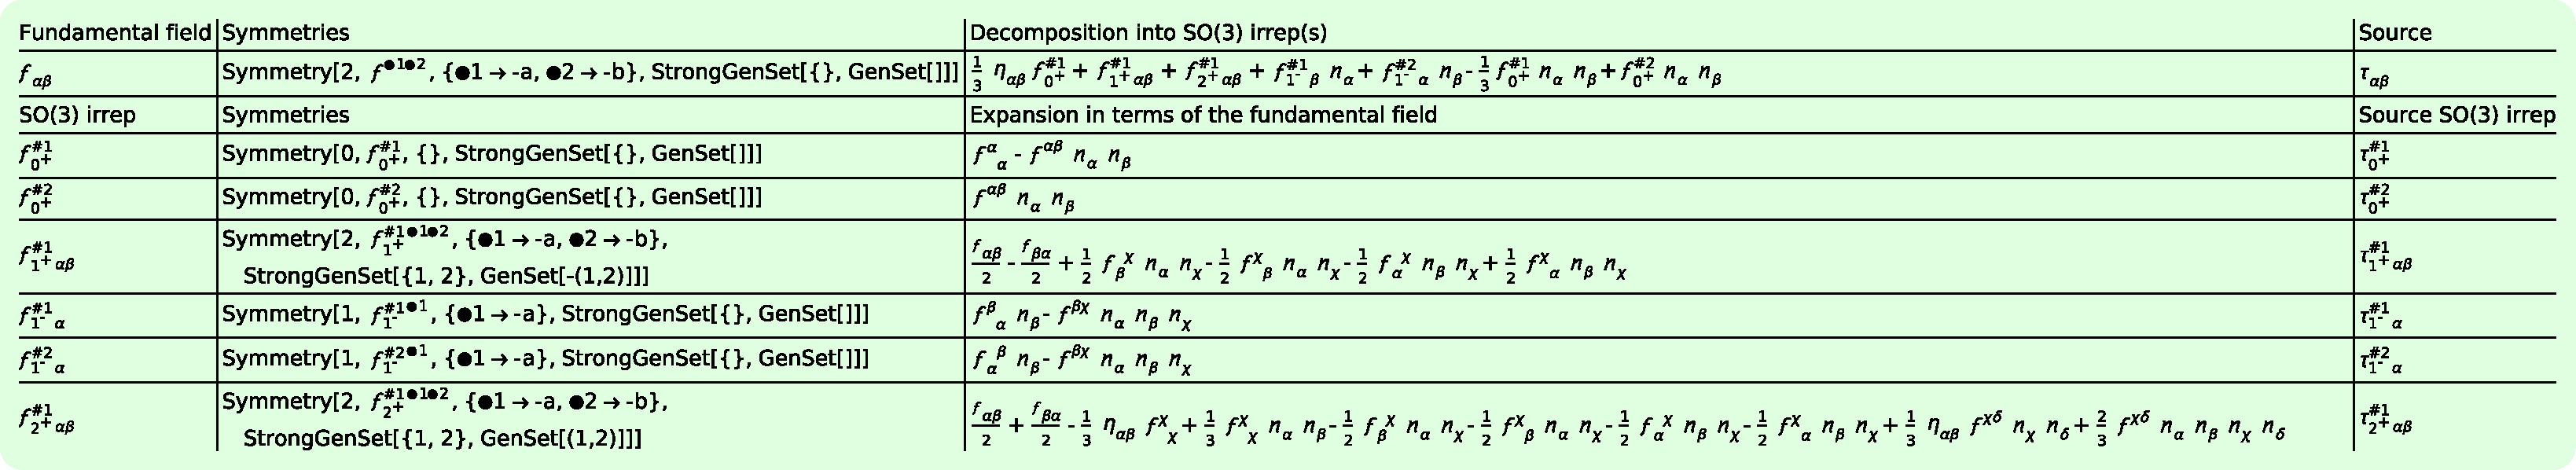
\includegraphics[width=\textwidth,height=\textheight,keepaspectratio]{FieldKinematicsF.pdf}
	\caption{\label{FieldKinematicsF} Kinematic structure of the tetrad perturbation~$\FieldPert{_{\mu\nu}}$, as used in~\cref{PGTAction,eWGTAction}. These definitions are used in~\crefrange{ParticleSpectrographGeneralCase}{ParticleSpectrographGeneralCasePGTNoVector}. See~\cite{Barker:2024juc} for further notational details. This is a vector graphic: all details are visible under magnification.}
\end{figure*}

\begin{figure*}[h]
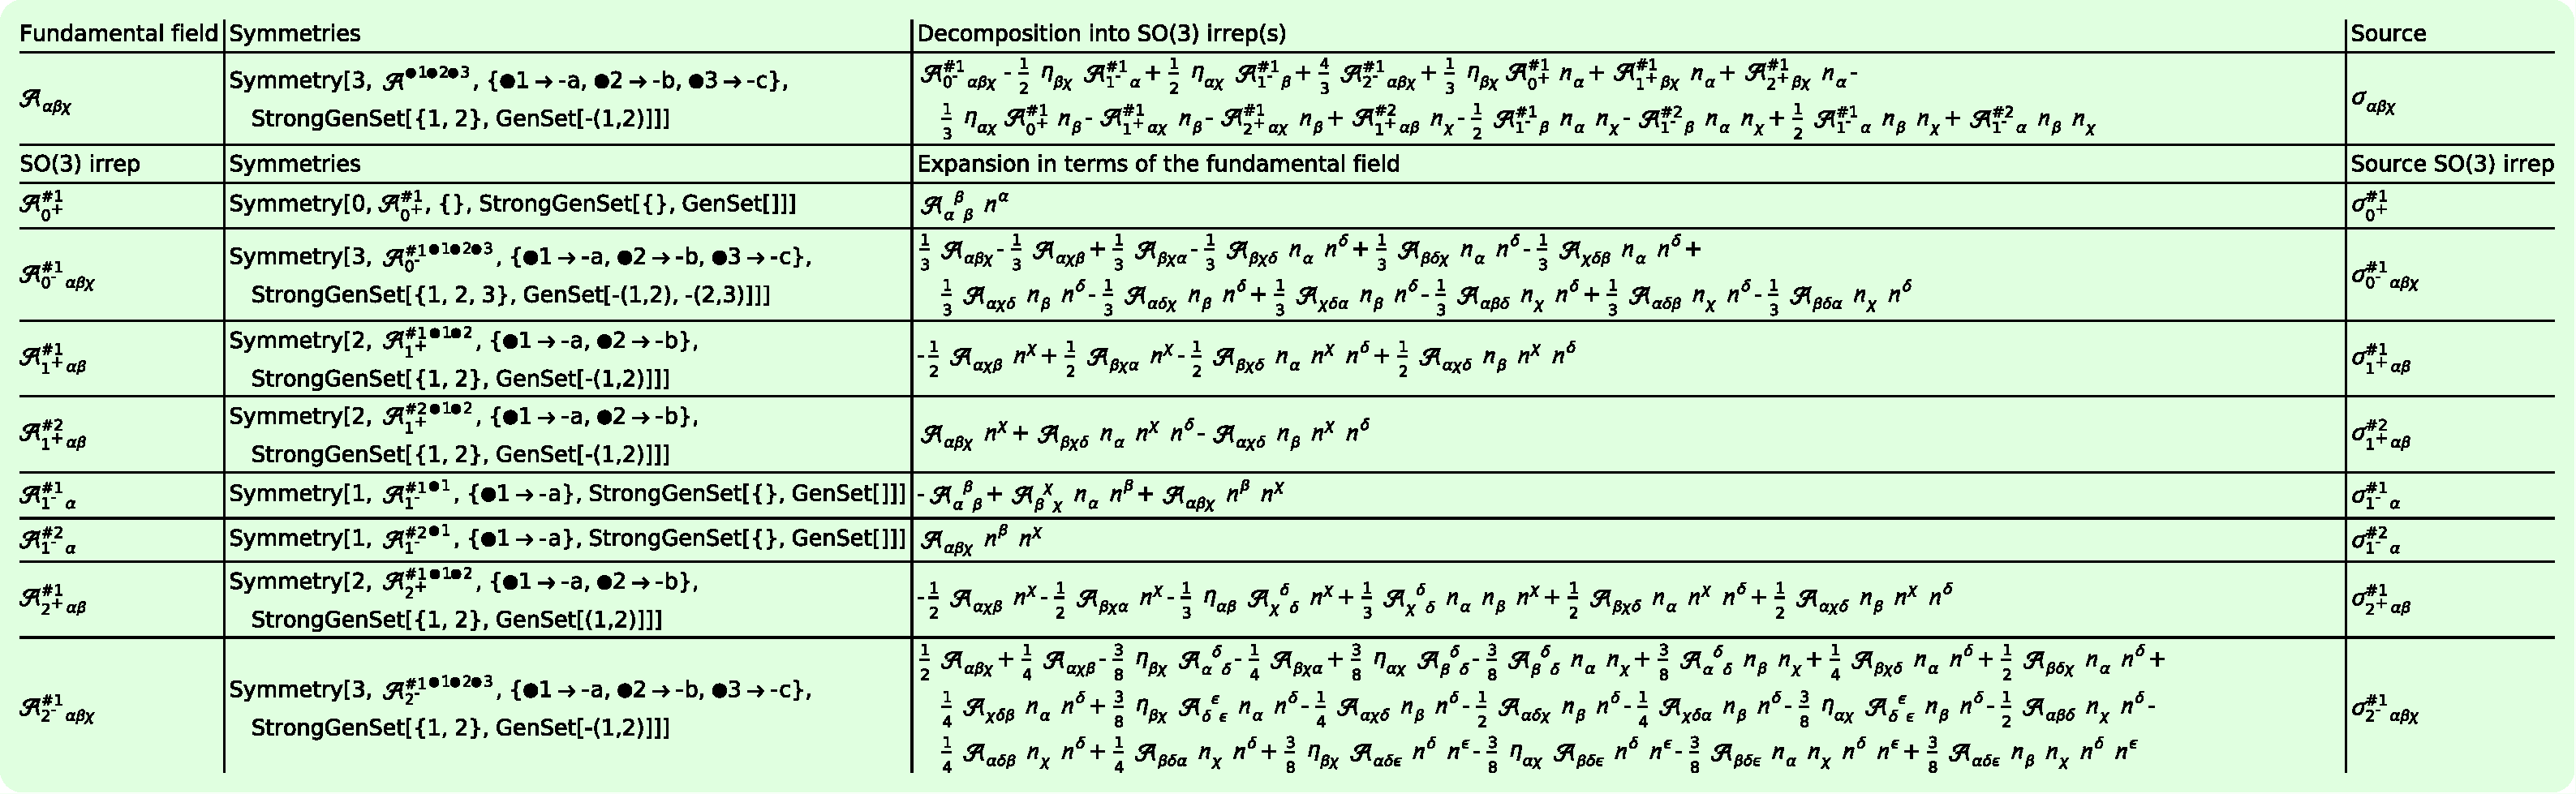
\includegraphics[width=\textwidth,height=\textheight,keepaspectratio]{FieldKinematicsA.pdf}
	\caption{\label{FieldKinematicsA} Kinematic structure of the spin connection perturbation~$\FieldA{_{\mu\nu\sigma}}$, as used in~\cref{PGTAction,eWGTAction}. Note that the~$2^-$ state has a hidden multi-term cyclic symmetry on all its indices, which is not accommodated by the C language implementation of the Butler--Portugal algorithm~\cite{Martin-Garcia:2008ysv}. These definitions are used in~\crefrange{ParticleSpectrographGeneralCase}{ParticleSpectrographGeneralCasePGTNoVector}. See~\cite{Barker:2024juc} for further notational details. This is a vector graphic: all details are visible under magnification.}
\end{figure*}

The particle spectra are obtained using the \emph{Particle Spectrum for Any Tensor Lagrangian} (\PSALTer{}) software~\cite{Barker:2023bmr,Barker:2024ydb,Barker:2024dhb,Barker:2024juc}. Recall that the kinematic variables of PGT were~$\big\{\FieldB{^i_\mu},\FieldA{^{ij}_\mu}\big\}$, and that the inverse~$\FieldH{_i^\mu}$ is determined by~$\FieldB{^i_\mu}$. This means that we are free to use~$\big\{\FieldH{_i^\mu},\FieldA{^{ij}_\mu}\big\}$ instead. Working in the weak-field regime, we take~$\FieldA{^{ij}_\mu}$ to be inherently perturbative. We define the exact perturbation~$\FieldH{_i^\mu}\equiv\FieldDelta{_i^\mu}+\FieldPert{_i^\mu}$, where we make the `Kronecker' choice of Minkowski vacuum (see alternative vacua~\cite{Barker:2023bmr,Blixt:2022rpl,Blixt:2023qbg}). There are a priori 16 d.o.f in~$\FieldPert{_i^\mu}$, and 24 d.o.f in~$\FieldA{^{ij}_\mu}$. Conjugate to~$\FieldPert{_i^\mu}$ and~$\FieldA{^{ij}_\mu}$ are the translational source (i.e. the asymmetric stress-energy tensor)~$\FieldTau{^i_\mu}$, and the matter spin current~$\FieldSpin{_{ij}^\mu}$~\cite{Rigouzzo:2023sbb,Rigouzzo:2022yan,Karananas:2021zkl}. To lowest order in the field perturbations, the Greek and Roman indices are interchangeable. For this reason the final set of fields used in the linearised analysis is~$\big\{\FieldPert{_{\mu\nu}},\FieldA{_{\mu\nu\sigma}}\big\}$, with conjugate sources~$\big\{\FieldTau{^{\mu\nu}},\FieldSpin{^{\mu\nu\sigma}}\big\}$. The various~$\mathrm{SO}(3)$ irreducible parts of these quantities are presented in~\cref{FieldKinematicsF,FieldKinematicsA}, and they have spin-parity ($J^P$) labels to identify them. Duplicate~$J^P$ states can arise, and these are distinguished by extra labels~$\#1$,~$\#2$, etc.

The actual analysis of the theory in~\cref{eWGTAction} was performed across 64 AMD\textsuperscript{\textregistered} \emph{Ryzen Threadripper} CPUs. For the completely unrestricted case in~\cref{eWGTAction} the mass expressions associated with the roots of the quartic pole are expected to be very cumbersome, so we abort the computation before they are computed: the structure of the wave operator and saturated propagator, without the mass spectrum, is shown in~\cref{ParticleSpectrographGeneralCase}. Before the evaluation of the `general' branch for which the~$k^4$ coefficient in~\cref{MasterConstraint} is removed, the condition~$\Alp{5}=\chi^2/\xi-2\left(\Alp{2}+2\Alp{4}\right)$ must be imposed on the linearised action. To avoid Lagrangian couplings appearing on the denominator of the linearised action\footnote{As a mild technical limitation, coupling coefficients in the denominator can cause \PSALTer{} to become slow.} we impose the constraint by introducing a new coupling~$\theta$ and setting in~\cref{eWGTAction}
\begin{equation}\label{Eliminations}
	\Alp{5}\mapsto\theta^2\xi-2\left(\Alp{2}+2\Alp{4}\right), \quad \chi\mapsto\theta\xi.
\end{equation}
The results are shown in~\cref{ParticleSpectrographGeneralCaseNoQuartic}, we see that apart from the two massless polarisations of the Einstein graviton, up to six torsion particles can propagate with the following square masses, where we eliminate~$\theta$ in terms of~$\chi$ and~$\xi$ using~\cref{Eliminations}
\begin{widetext}
\begin{subequations}
\begin{align}
	\MassSquared{0^+}&\equiv\frac{\MPl{}^2\left(2\Bet{1}+\Bet{2}+3\Bet{3}+\MPl{}^2\right)}{2\left(2\Bet{1}+\Bet{2}+3\Bet{3}\right)\left(6\Alp{1}+2\Alp{3}-2\Alp{4}+2\Alp{6}+\chi^2/\xi\right)},\label{Mass0p}\\
	\MassSquared{0^-}&\equiv-\frac{8\Bet{1}-8\Bet{2}+\MPl{}^2}{4\Alp{2}+12\Alp{4}-2\chi^2/\xi},\label{Mass0m}\\
	\MassSquared{1^+}&\equiv\frac{-32\Bet{1}^2+16\Bet{2}^2-10\Bet{2}\MPl{}^2+\MPl{}^4+4\Bet{1}\left(4\Bet{2}+\MPl{}^2\right)}{4\left(\Alp{2}-\Alp{3}+4\Alp{4}-4\Alp{6}\right)\left(2\Bet{1}-\Bet{2}\right)} ,\label{Mass1p}\\
	\MassSquared{1^-}&\equiv-\frac{24\left(4\Bet{1}+2\Bet{2}-\MPl{}^2\right)\left(2\Bet{1}+\Bet{2}+3\Bet{3}+\MPl{}^2\right)}{\xi\left(48\Bet{3}\chi^3/\xi^3+4\Bet{1}\left(1+8\chi/\xi+24\chi^2/\xi^2\right)+2\Bet{2}\left(1+8\chi/\xi+24\chi^2/\xi^2\right)-\MPl{}^2-8\MPl{}^2\chi/\xi\right)},\label{Mass1m}\\
	\MassSquared{2^+}&\equiv\frac{\left(4\Bet{1}+2\Bet{2}-\MPl{}^2\right)\MPl{}^2}{4\left(2\Bet{1}+\Bet{2}\right)\left(3\Alp{2}-\Alp{3}+4\Alp{4}-4\Alp{6}-2\chi^2/\xi\right)},\label{Mass2p}\\
	\MassSquared{2^-}&\equiv\frac{4\Bet{1}+2\Bet{2}-\MPl{}^2}{4\Alp{2}-2\chi^2/\xi}.\label{Mass2m}
\end{align}
\end{subequations}
\end{widetext}
By adding up the~$1+1+3+3+5+5$ spin multiplicities of~\crefrange{Mass0p}{Mass2m} we recover the~$16+24$ kinematic d.o.f in~$\big\{\FieldB{^i_\mu},\FieldA{^{ij}_\mu}\big\}$, less the~$2\times(4+6)$ gauge d.o.f associated with Poincar\'e gauge symmetry --- the only surviving symmetry of the embedded theory. The branch~$2\Alp{2}+4\Alp{4}+\Alp{5}=\chi=0$ is likewise found by setting~$\Alp{5}\mapsto-2\left(\Alp{2}+2\Alp{4}\right)$ and~$\chi\mapsto 0$ in~\cref{eWGTAction}. The analysis is presented in~\cref{ParticleSpectrographGeneralCaseNoQuarticSplit}, and shows that the mass spectrum is fully consistent with imposing~$\chi\mapsto 0$ in~\crefrange{Mass0p}{Mass2m}. Finally, the case~$\xi=\chi=0$ in~\cref{eWGTAction} without any further restrictions leads in~\cref{ParticleSpectrographGeneralCasePGT} to the general case of PGT in~\cref{PGTAction}, which was found previously in~\cite{Hayashi:1980qp}, namely
\begin{widetext}
\begin{subequations}
\begin{align}
	\MassSquared{0^+}&\equiv\frac{\MPl{}^2\left(2\Bet{1}+\Bet{2}+3\Bet{3}+\MPl{}^2\right)}{2\left(6\Alp{1}+2\Alp{2}+2\Alp{3}+2\Alp{4}+\Alp{5}+2\Alp{6}\right)\left(2\Bet{1}+\Bet{2}+3\Bet{3}\right)},\label{NewMass0p}\\
	\MassSquared{0^-}&\equiv-\frac{8\Bet{1}-8\Bet{2}+\MPl{}^2}{4\Alp{4}-2\Alp{5}},\label{NewMass0m}\\
	\MassSquared{1^-}&\equiv-\frac{\left(4\Bet{1}+2\Bet{2}-\MPl{}^2\right)\left(2\Bet{1}+\Bet{2}+3\Bet{3}+\MPl{}^2\right)}{2\left(2\Alp{2}+4\Alp{4}+\Alp{5}\right)\left(2\Bet{1}+\Bet{2}+\Bet{3}\right)},\label{NewMass1m}\\
	\MassSquared{2^+}&\equiv\frac{\MPl{}^2\left(-4\Bet{1}-2\Bet{2}+\MPl{}^2\right)}{4\left(\Alp{2}+\Alp{3}+4\Alp{4}+2\Alp{5}+4\Alp{6}\right)\left(2\Bet{1}+\Bet{2}\right)},\label{NewMass2p}\\
	\MassSquared{2^-}&\equiv\frac{-4\Bet{1}-2\Bet{2}+\MPl{}^2}{2\left(4\Alp{4}+\Alp{5}\right)}.\label{NewMass2m}
\end{align}
\end{subequations}
\end{widetext}
Whilst we confirmed already that the~$\chi\to 0$ limit of~\crefrange{Mass0p}{Mass2m} was continuous, it is evident from~\cref{Mass1m} that once~$\chi\to 0$ has been taken the limit~$\xi\to 0$ eliminates the~$1^-$ vector in which we have been so interested. In fact, this is not surprising, because taking~$\chi\to 0$ at finite~$\xi$ corresponds to setting~$2\Alp{2}+4\Alp{4}+\Alp{5}=0$. From~\cref{NewMass1m} we see how this latter condition would equivalently kill the~$1^-$ mode in~\cref{PGTAction} (we confirm this in~\cref{ParticleSpectrographGeneralCasePGTNoVector}), and the~\cref{PGTAction} theory-space is reached by~$\xi\to 0$.

\begin{figure*}[ht]
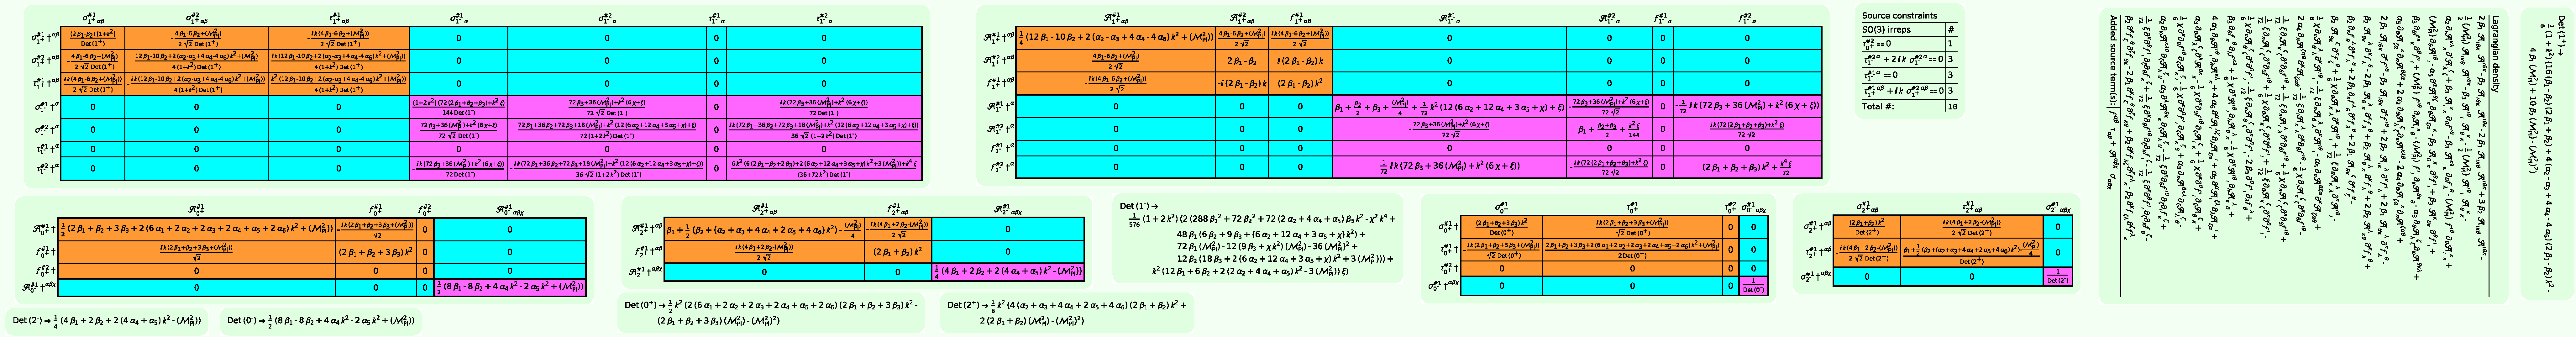
\includegraphics[width=\textwidth]{ParticleSpectrographGeneralCase.pdf}
	\caption{\label{ParticleSpectrographGeneralCase} Partial particle spectrograph of the completely general theory in~\cref{eWGTAction}. From the~$1^-$ sector of the saturated propagator we may read off the quartic pole in~\cref{MasterConstraint}. All quantities are defined in~\cref{FieldKinematicsF,FieldKinematicsA}. See~\cite{Barker:2024juc} for further notational details. This is a vector graphic: all details are visible under magnification.}
\end{figure*}
\begin{figure*}[ht]
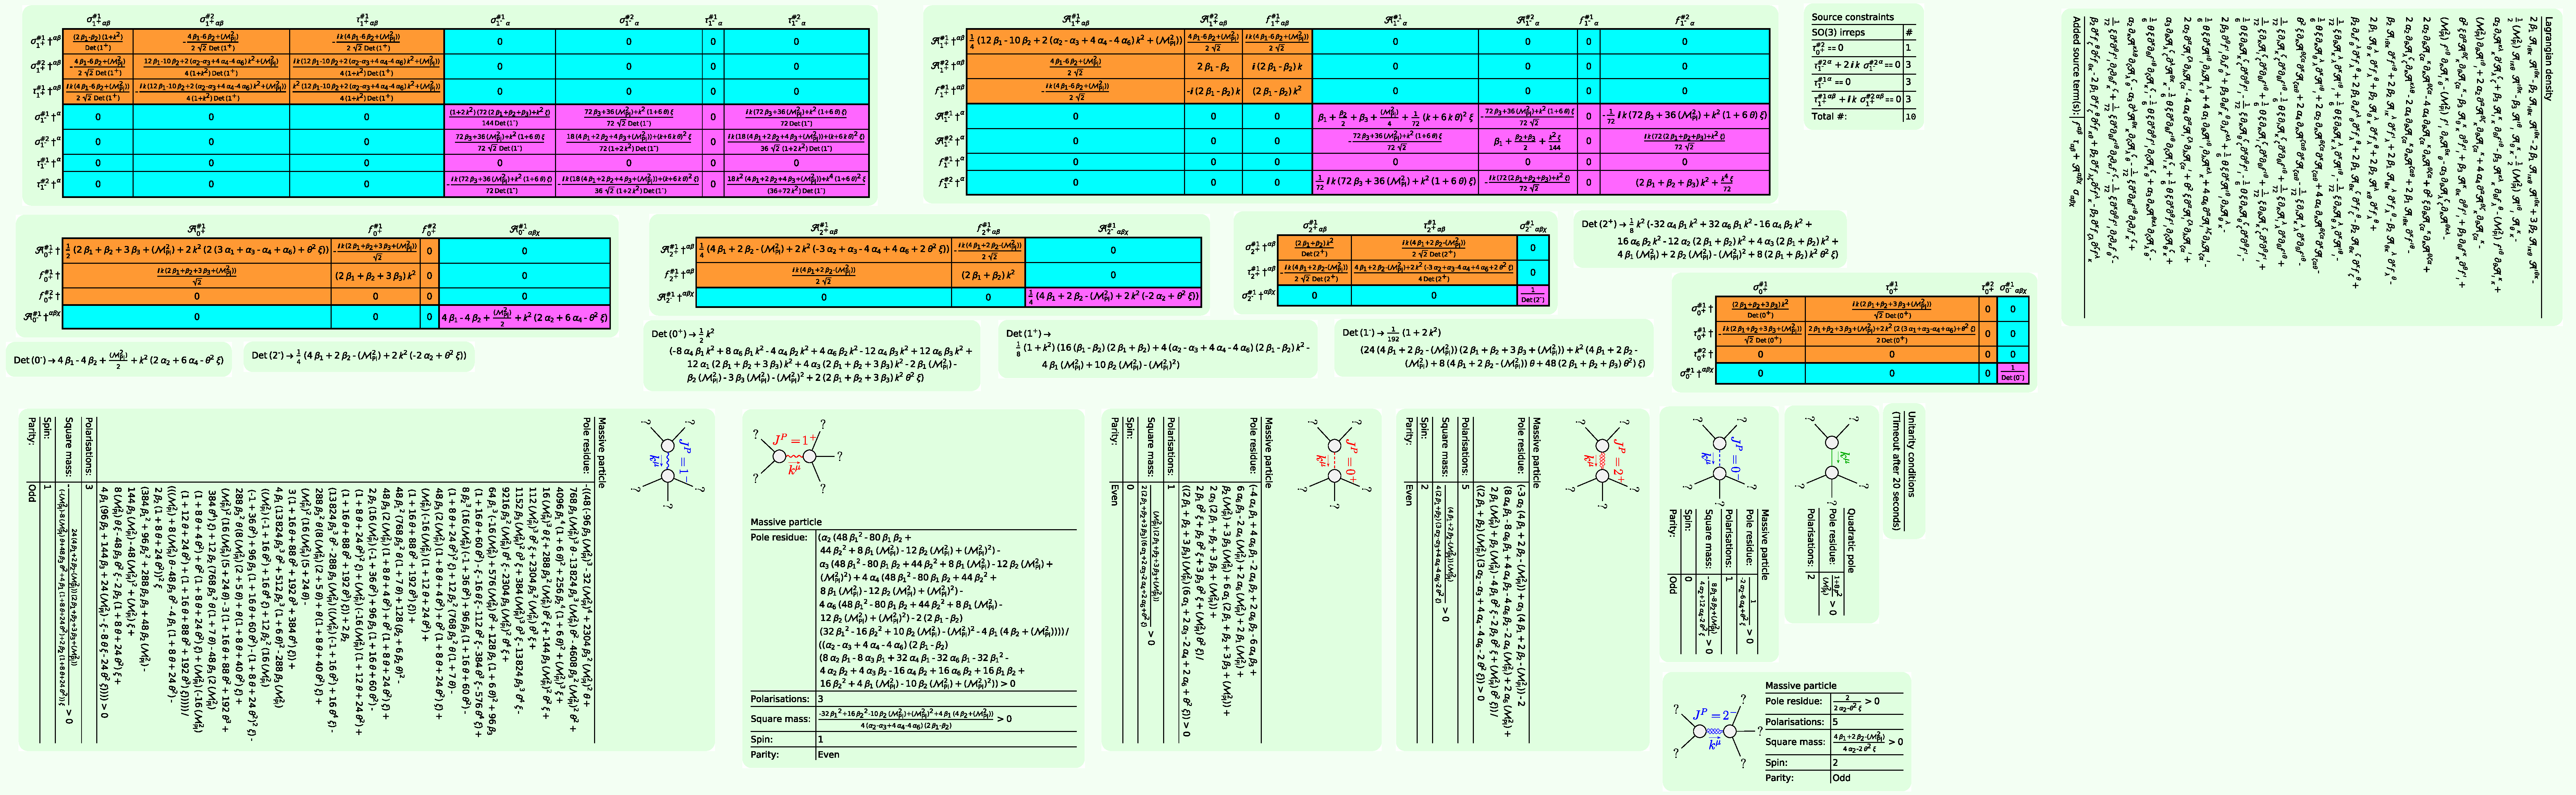
\includegraphics[width=\textwidth]{ParticleSpectrographGeneralCaseNoQuartic.pdf}
	\caption{\label{ParticleSpectrographGeneralCaseNoQuartic} Particle spectrograph of the branch~$\Alp{5}=\chi^2/\xi-2\left(\Alp{2}+2\Alp{4}\right)$ of~\cref{eWGTAction}, which gives rise to the mass spectra in~\crefrange{Mass0p}{Mass2m}. All quantities are defined in~\cref{FieldKinematicsF,FieldKinematicsA,Eliminations}. See~\cite{Barker:2024juc} for further notational details. This is a vector graphic: all details are visible under magnification.}
\end{figure*}
\begin{figure*}[ht]
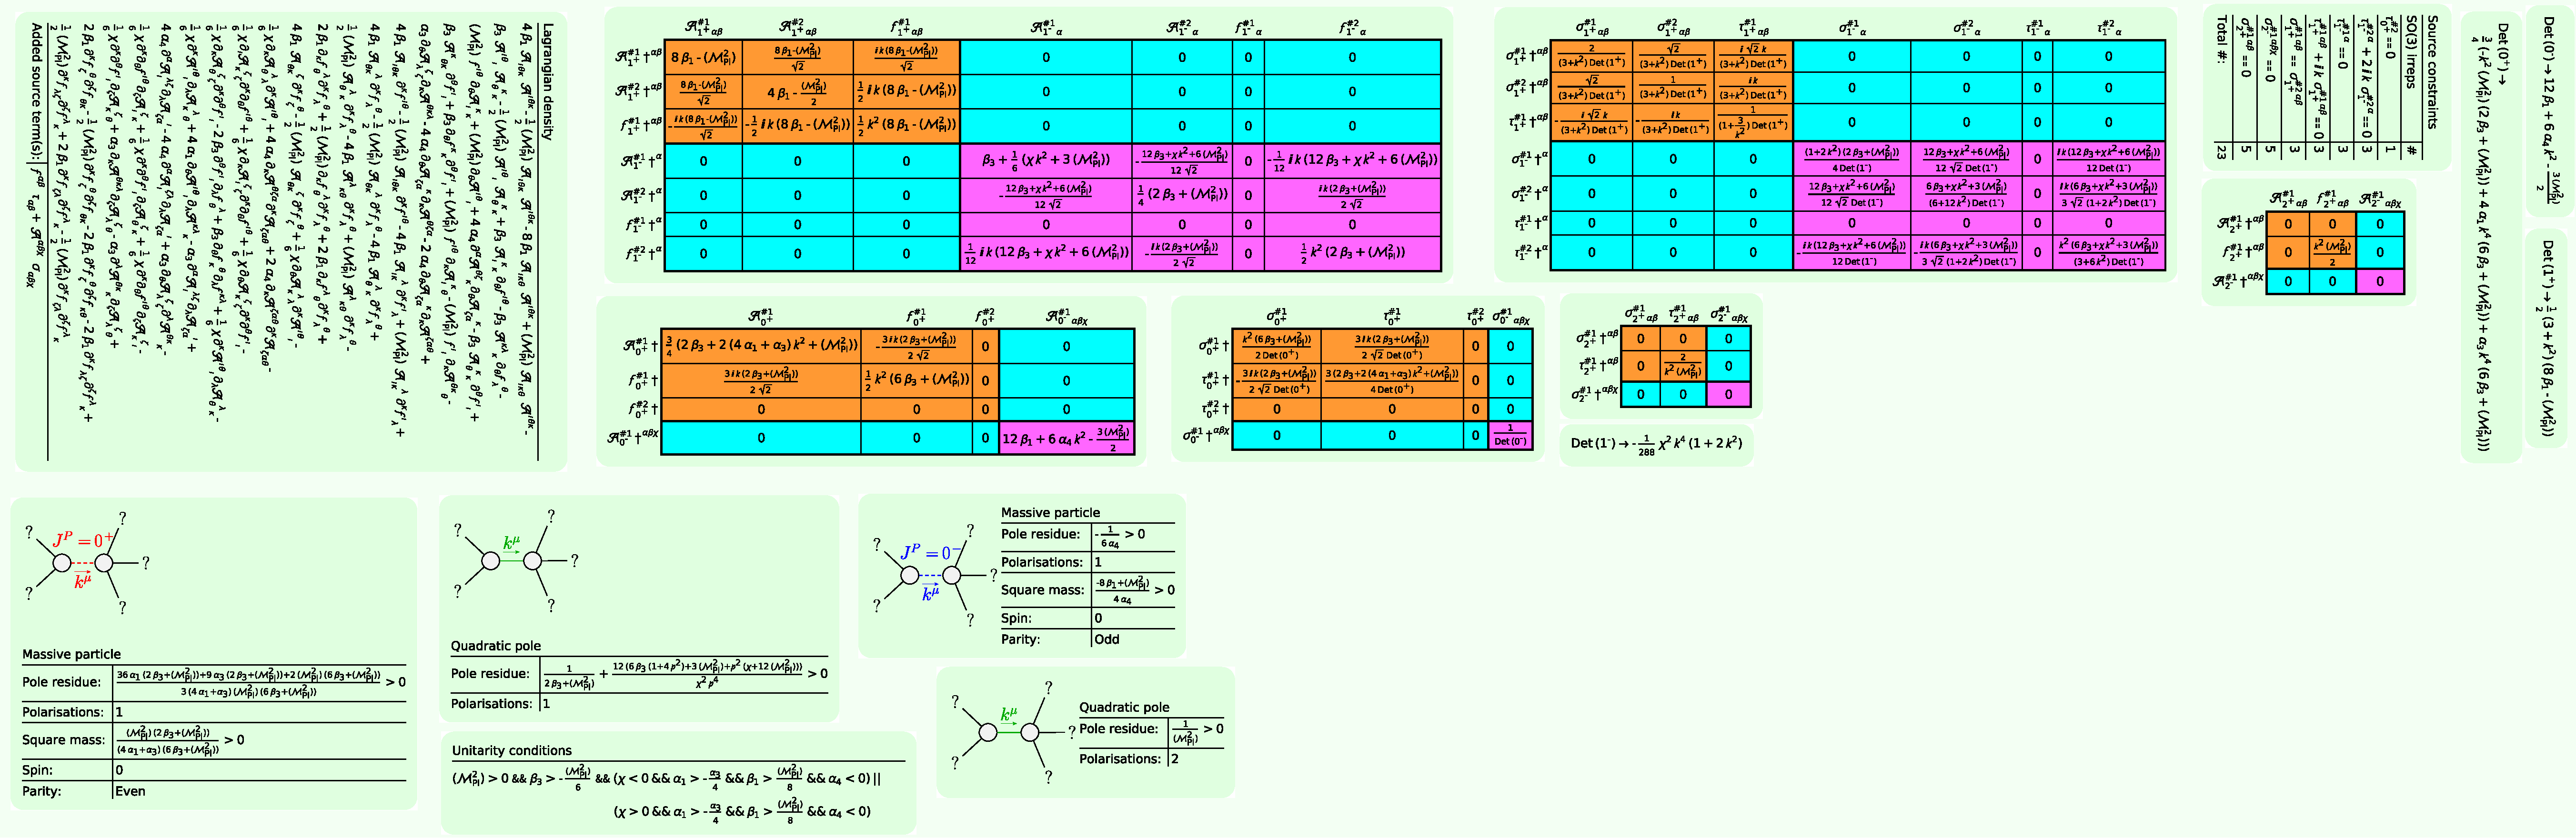
\includegraphics[width=\textwidth]{ParticleSpectrographBranch1Conservative.pdf}
	\caption{\label{ParticleSpectrographBranch1Conservative} Particle spectrograph of the branch~$\Alp{2}=\Alp{3}-4\Alp{4}+\Alp{6}=4\Alp{4}+\Alp{5}=4\Bet{1}+2\Bet{2}-\MPl{}^2=0$ of~\cref{eWGTAction}. All quantities are defined in~\cref{FieldKinematicsF,FieldKinematicsA}. See~\cite{Barker:2024juc} for further notational details. This is a vector graphic: all details are visible under magnification.}
\end{figure*}
\begin{figure*}[ht]
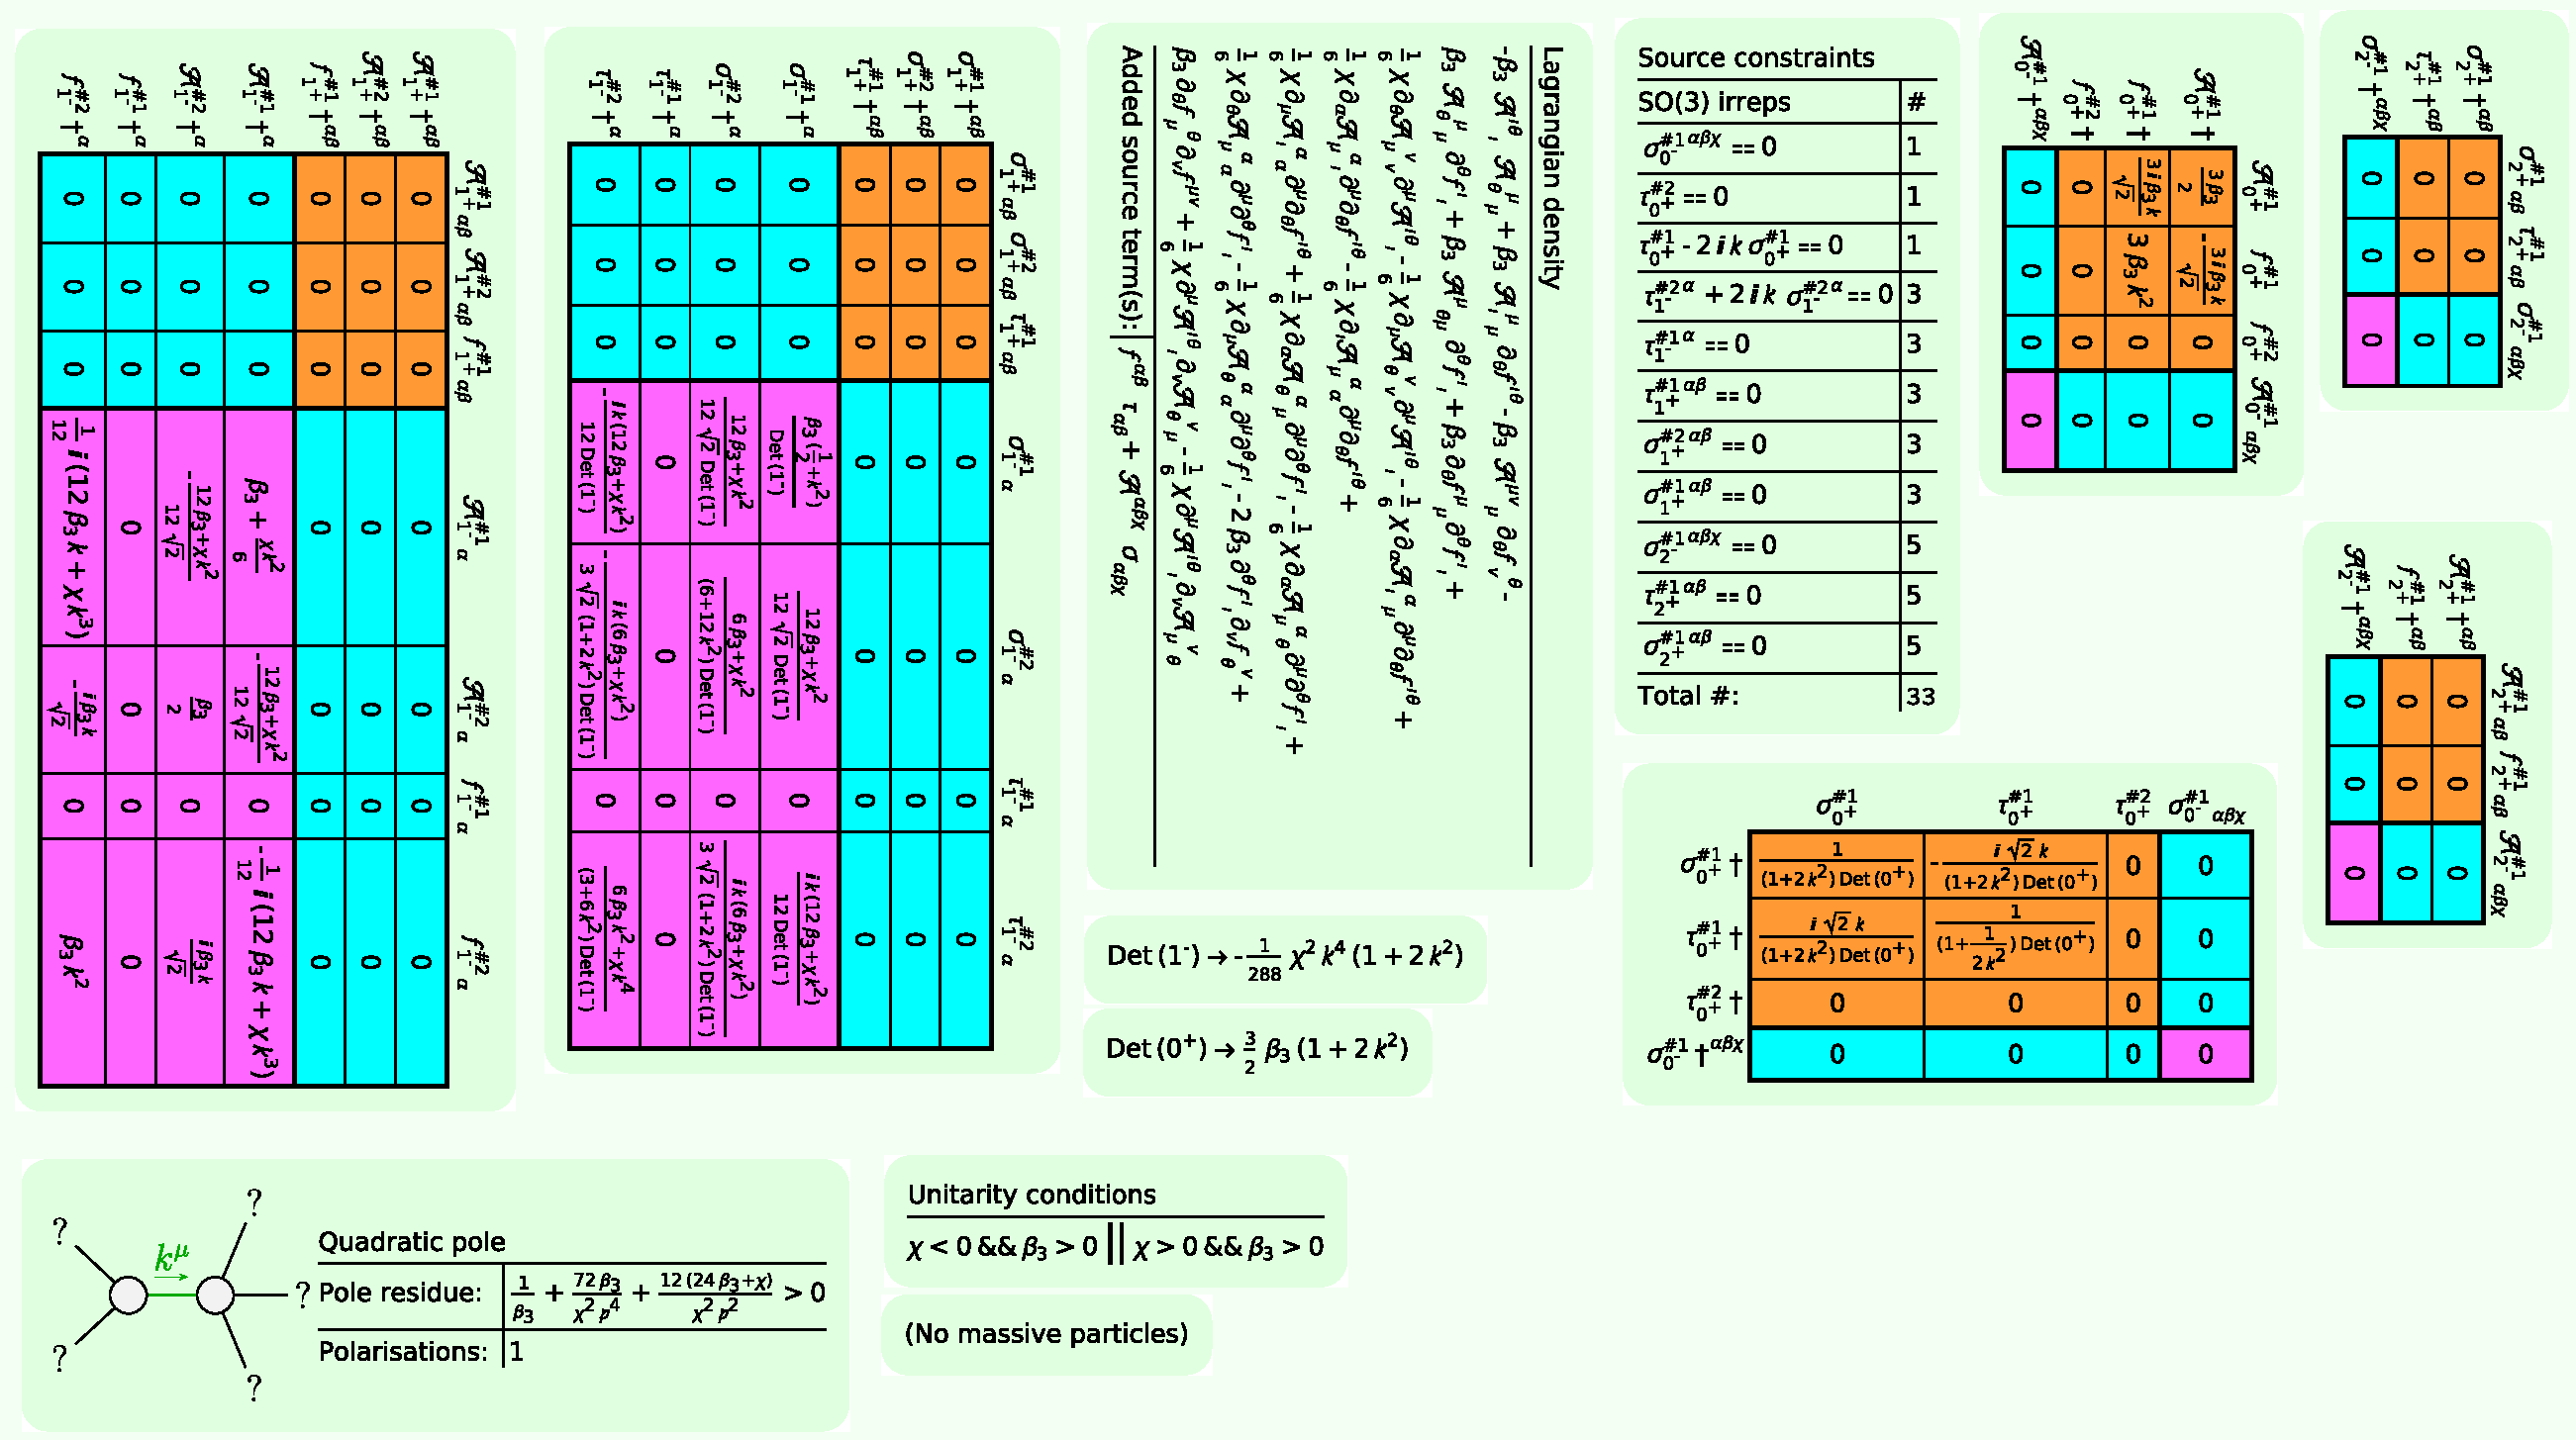
\includegraphics[width=\textwidth]{ParticleSpectrographSwitchonPGT.pdf}
	\caption{\label{ParticleSpectrographSwitchonPGT} Particle spectrograph of~\cref{SwitchonPGT}, i.e. the minimal PGT realisation of the novel massless scalar particle which appears in~\cref{ParticleSpectrographBranch1Conservative}. All quantities are defined in~\cref{FieldKinematicsF,FieldKinematicsA}. See~\cite{Barker:2024juc} for further notational details. This is a vector graphic: all details are visible under magnification.}
\end{figure*}
\begin{figure*}[ht]
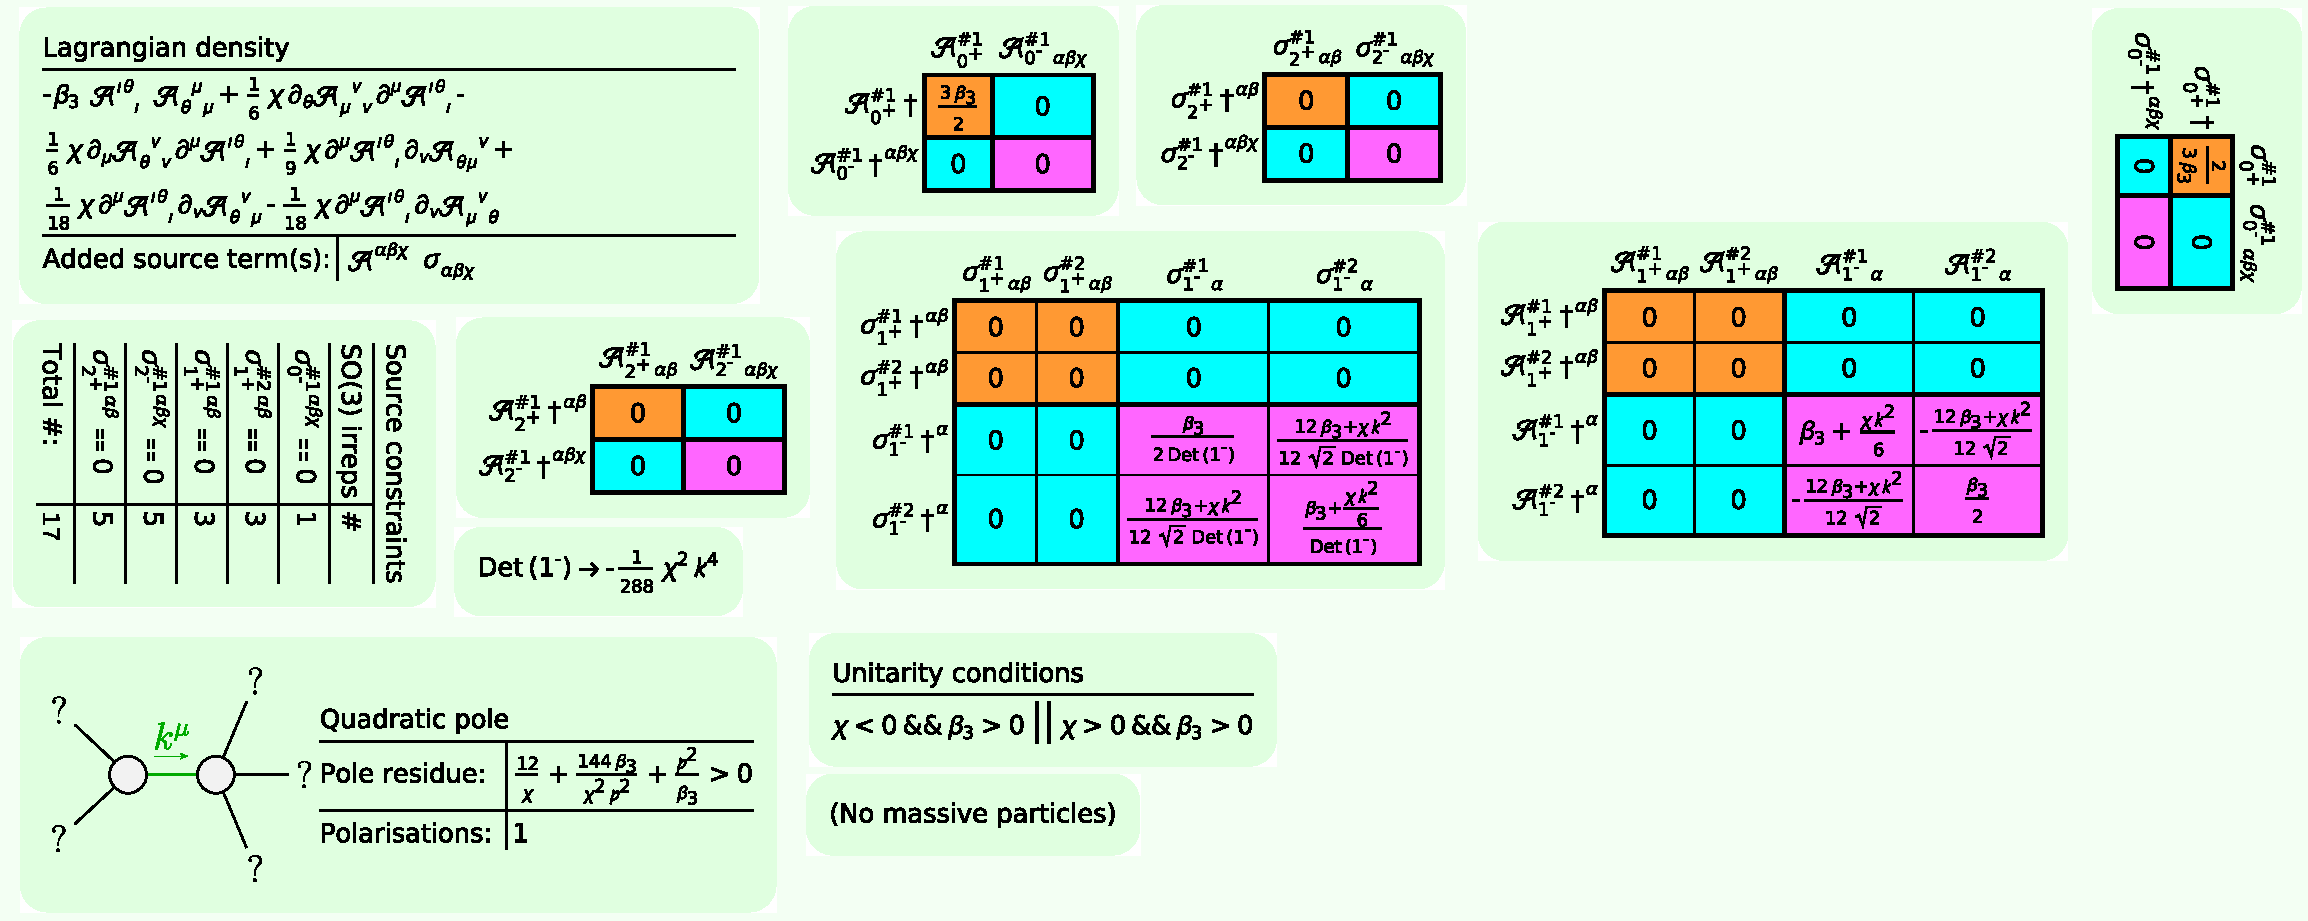
\includegraphics[width=\textwidth]{ParticleSpectrographSwitchonNoAxialVector.pdf}
	\caption{\label{ParticleSpectrographSwitchonNoAxialVector} Particle spectrograph of~\cref{NewCurtright}, i.e. the minimal model of the novel scalar particle which appears in~\cref{ParticleSpectrographBranch1Conservative,ParticleSpectrographSwitchonPGT}. We use the rotational gauge field perturbation~$\FieldA{_{\mu\nu\sigma}}\equiv\FieldA{_{[\mu\nu]\sigma}}$ as a proxy for the Curtright field~$\Curtright{_{\mu\nu\sigma}}\equiv\Curtright{_{[\mu\nu]\sigma}}$ with~$\Curtright{_{[\mu\nu\sigma]}}\equiv 0$, because the latter multi-term symmetry is a difficult attribute to declare in the \PSALTer{} framework. It can be confirmed (by applying transformation rules to the Lagrangian density in this figure, and repeating the analysis) that the axial part~$\FieldA{_{[\mu\nu\sigma]}}$ does \emph{not} contribute to the spectrum. All quantities are defined in~\cref{FieldKinematicsF,FieldKinematicsA}. See~\cite{Barker:2024juc} for further notational details. This is a vector graphic: all details are visible under magnification.}
\end{figure*}
\begin{figure*}[ht]
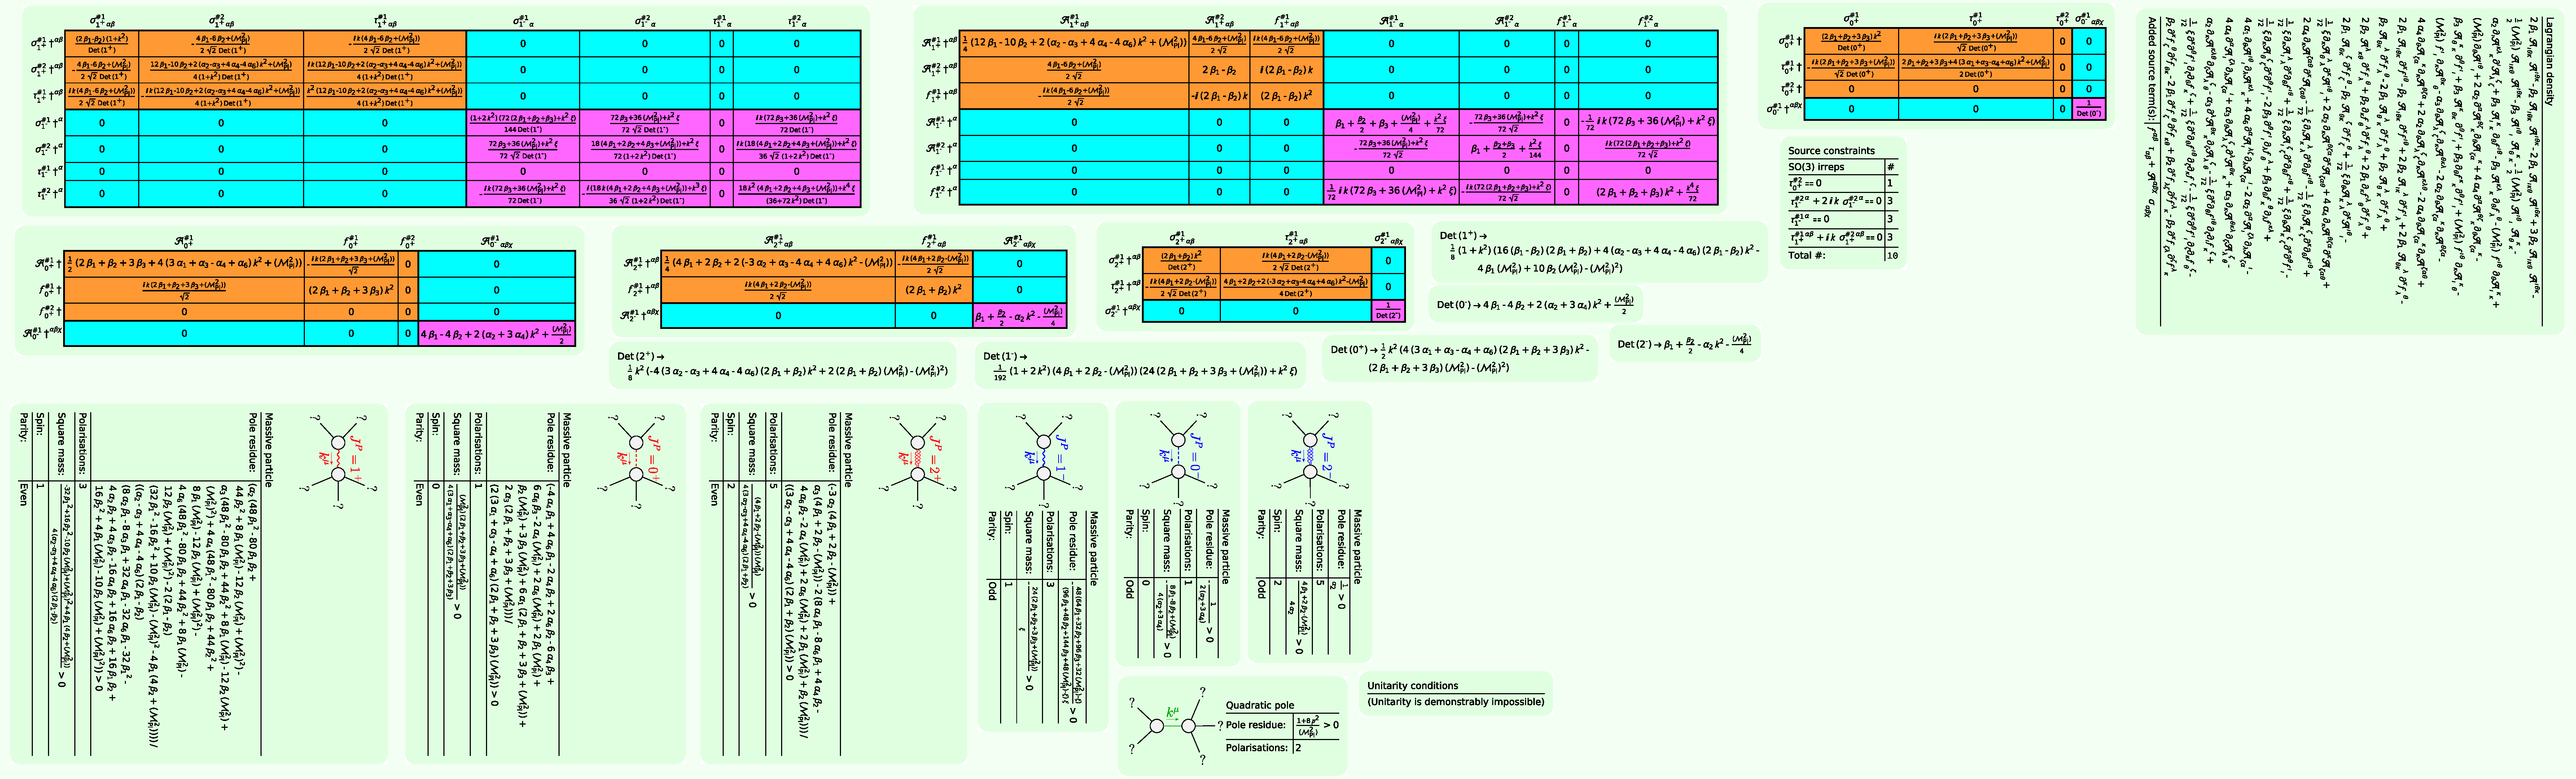
\includegraphics[width=\textwidth]{ParticleSpectrographGeneralCaseNoQuarticSplit.pdf}
	\caption{\label{ParticleSpectrographGeneralCaseNoQuarticSplit} Particle spectrograph of the branch~$\Alp{5}=-2\left(\Alp{2}+2\Alp{4}\right)$ with~$\chi=0$ of~\cref{eWGTAction}, which gives rise to the~$\chi\mapsto 0$ limit of the mass spectra in~\crefrange{Mass0p}{Mass2m} (see~\cref{ParticleSpectrographGeneralCaseNoQuartic}). All quantities are defined in~\cref{FieldKinematicsF,FieldKinematicsA,Eliminations}. See~\cite{Barker:2024juc} for further notational details. This is a vector graphic: all details are visible under magnification.}
\end{figure*}
\begin{figure*}[ht]
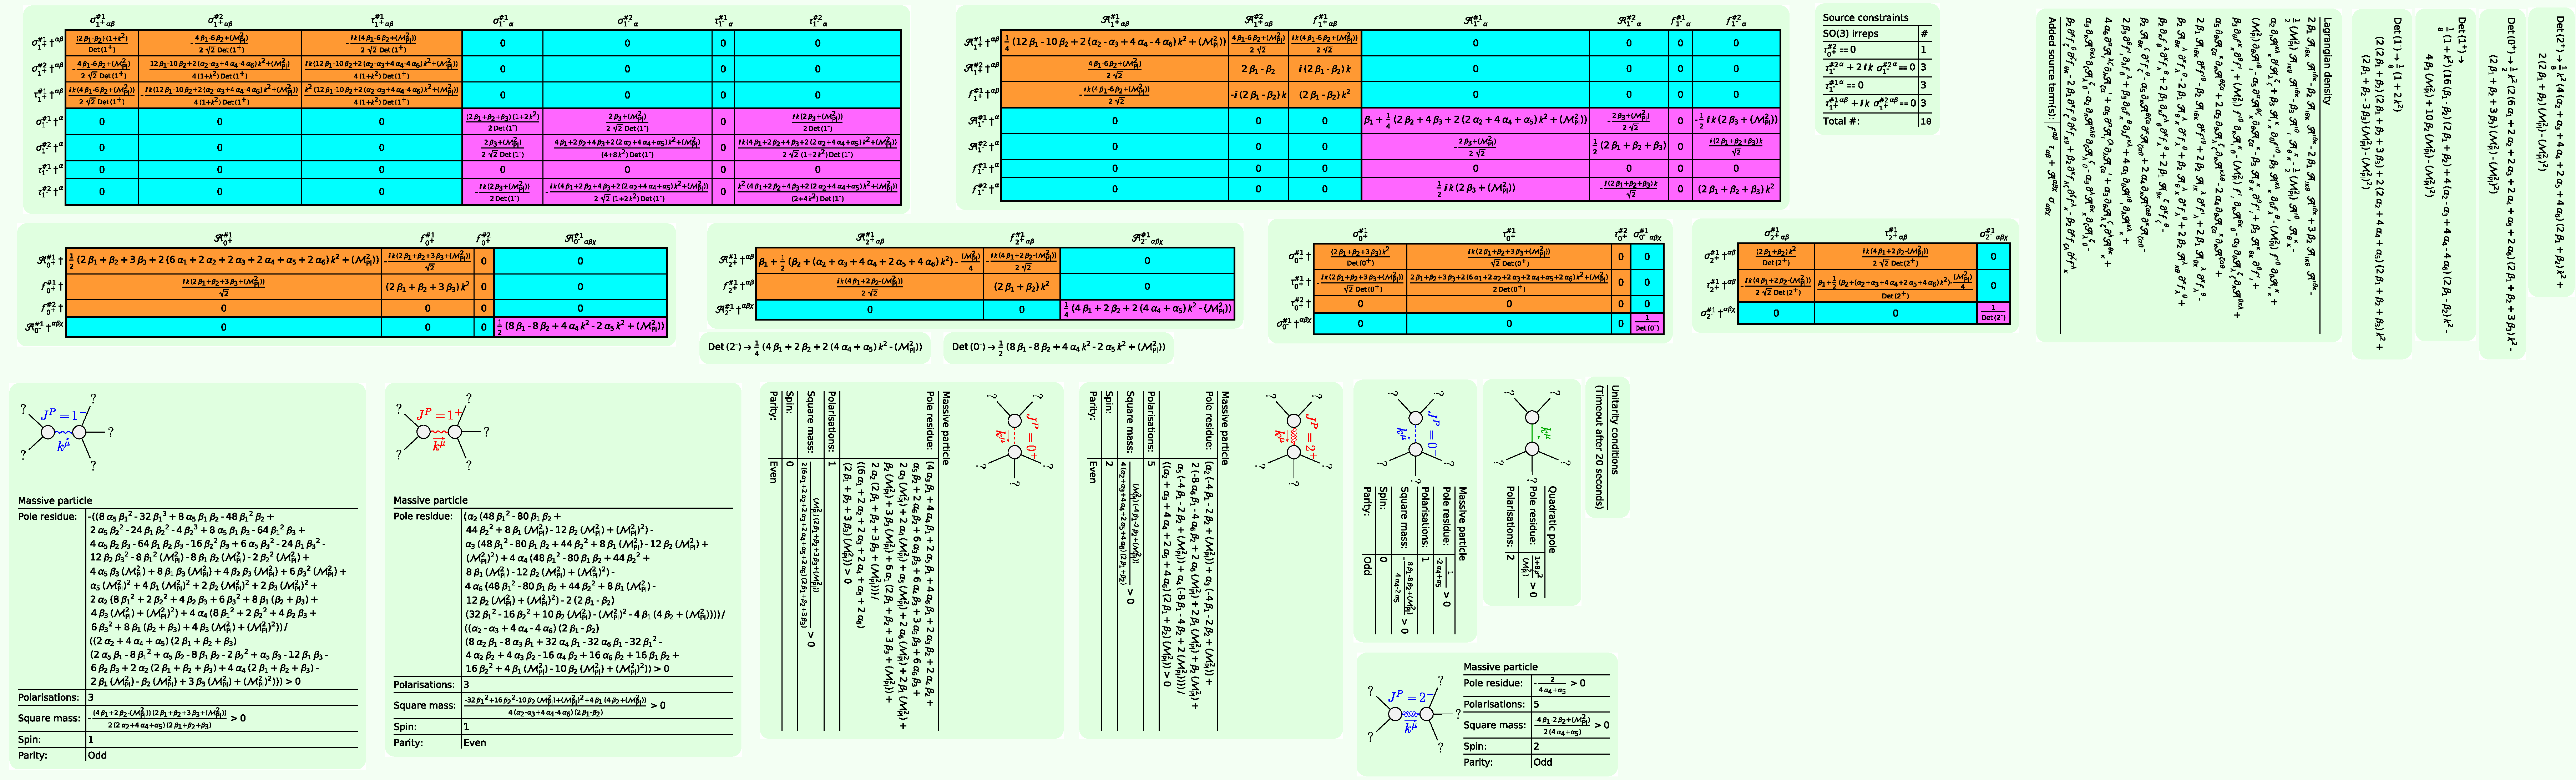
\includegraphics[width=\textwidth]{ParticleSpectrographGeneralCasePGT.pdf}
	\caption{\label{ParticleSpectrographGeneralCasePGT} Particle spectrograph of the branch~$\xi=\chi=0$ of~\cref{eWGTAction}, which gives rise to the mass spectra in~\crefrange{NewMass0p}{NewMass2m}, as first presented in~\cite{Hayashi:1980qp}. All quantities are defined in~\cref{FieldKinematicsF,FieldKinematicsA}. See~\cite{Barker:2024juc} for further notational details. This is a vector graphic: all details are visible under magnification.}
\end{figure*}
\begin{figure*}[ht]
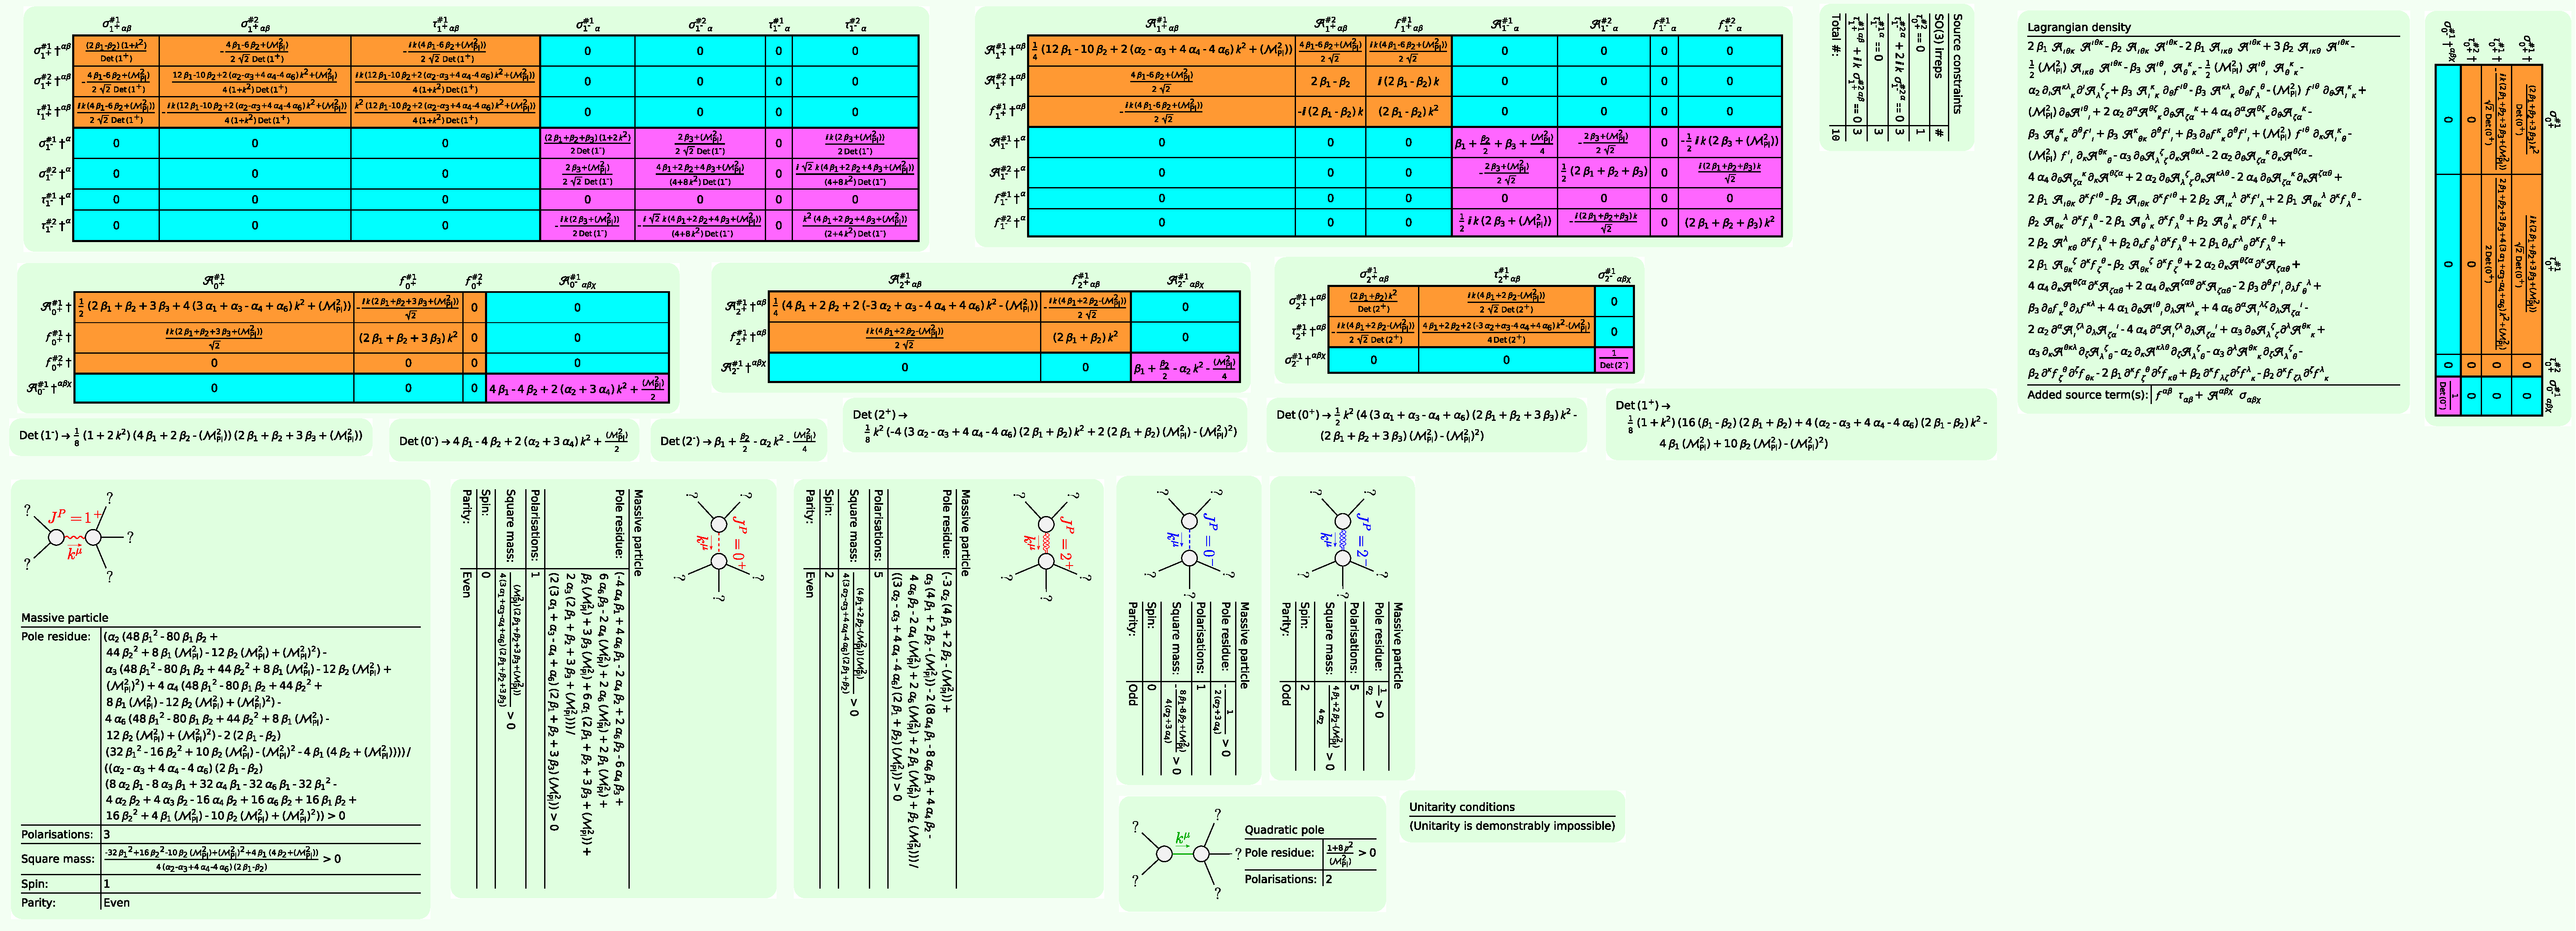
\includegraphics[width=\textwidth]{ParticleSpectrographGeneralCasePGTNoVector.pdf}
	\caption{\label{ParticleSpectrographGeneralCasePGTNoVector} Particle spectrograph of the branch~$\Alp{5}=-2\left(\Alp{2}+2\Alp{4}\right)$ of~\cref{PGTAction}, confirming that the~$1^-$ mode is removed. All quantities are defined in~\cref{FieldKinematicsF,FieldKinematicsA}. See~\cite{Barker:2024juc} for further notational details. This is a vector graphic: all details are visible under magnification.}
\end{figure*}

\end{document}
